
\documentclass{gist}

\def\putepsf#1{\centering \parbox{14cm}{\epsfxsize = 14cm \epsfbox{#1}}}
\usepackage{graphicx}

\usepackage{amsmath, amssymb}

\usepackage{booktabs}

% \usepackage{algorithm}
% \usepackage{amsfonts}
% \usepackage{algorithmic}
\AtBeginEnvironment{algorithm}{\setstretch{1.0}}
\usepackage[lofdepth=1]{subfig}
\usepackage[rightcaption]{sidecap}
\usepackage{multirow}
\usepackage{makecell}
% \usepackage{array}

% yoon
\usepackage[ruled,vlined,linesnumbered]{algorithm2e}
\usepackage{etoolbox}
\usepackage{url}

\newcommand\etal{\textit{et~al.\ }}
\newcommand\eg{\textit{e.g.\ }}
\newcommand\ie{\textrm{i.e.\ }}
\newcommand\R{\mathbb{R}}
% yoon

% \usepackage{theorem}
\usepackage{setspace}
\usepackage{appendix}
\usepackage{cite}
\usepackage{csquotes}

\usepackage[colorlinks=true,linkcolor=black,citecolor=black]{hyperref}
% \usepackage[]{hyperref}
% \hypersetup{
%     % bookmarksnumbered=true,
%     %   linkbordercolor=blue,
%     %   filebordercolor=red,
%     %   citebordercolor = green,      
%     %   urlbordercolor=red,
%       %
%       colorlinks=false
%       % linkcolor=blue,
%       % filecolor=blue,
%       % citecolor = blue,      
%       % urlcolor=cyan,
% }

\usepackage{bookmark}
\bookmarksetup{numbered}

\makeatletter
\bookmarksetup{%
  addtohook={%
    \ifnum\toclevel@chapter=\bookmarkget{level}\relax
      \renewcommand*{\numberline}[1]{CHAPTER #1 }%
    \fi
  },
}
\makeatother

\usepackage{cleveref}
% autonum hides the equation numbers if they are not referenced.
% \usepackage{autonum}

\usepackage{amsthm}
\newtheorem{theorem}{Theorem}[section]
\newtheorem{lemma}{Lemma}[section]
\newtheorem{corollary}{Corollary}[section]
\newtheorem{proposition}{Proposition}[section]
\newtheorem{assumption}{Assumption}[section]
\theoremstyle{remark}
\newtheorem{remark}{Remark}[section]
\theoremstyle{definition}
\newtheorem{definition}{Definition}[section]

%-----------------------------------------------------------------------
% Department code list
% IC - Information and Communications
% IM - Information and Mechatronics
% EC - Electric Engineering and Computer Science
% MS - Materials Science and Engineering
% ME - Mechanical and Robotics Engineering
% AI - Artificial Intelligence Graduate School
% EN - Earth Science and Environmental Engineering
% LS - Life Science
% PH - Physics and Photon Science
% CH - Chemistry
% NA - Nanobio Materials and Electronics
% MD - Biomedical Science and Engineering
% ET - Integrated Technology 에너지 융합 학제
% CT - Integrated Technology 문화기술 융합 학제
% RT - Integrated Technology 지능로봇프로그램

% Department code
%\code{{BS/}{EC}}
%\code{{MS/}{EC}} % 학위와 소속 코드, 초록 페이지에 나타남
\code{{MS/}{AI}}
%-----------------------------------------------------------------------
% Thesis title in English
% Insert \titlebreak where lines are to be separated.  Do not use the LaTeX command '\\'.

%\etitle{Study on Image Segmentation and Action Recognition in Computer Vision}

\etitle{State-wise Safety in Autonomous Driving \titlebreak via Lagrangian-based \titlebreak Constrained Reinforcement Learning}

%\etitle{Study on Segmentation and Recognition for an Image Understanding}
%\etitle{Genetic Programming: \titlebreak New Optimization Tools for Real-World Applications}

%-----------------------------------------------------------------------
% Thesis title in Korean
% Insert \titlebreak where lines are to be separated.  Do not use the LaTeX command '\\'.
%\begin{spacing}{2.0}
\ktitle{라그랑지안 기반 제약 강화학습을 이용한 자율주행에서의 상태별 안전성 고려}
%\end{spacing}
%-----------------------------------------------------------------------
% Advisor's name in English without a position such as 'Prof.'.
\advisor{Ue-Hwan Kim}

%-----------------------------------------------------------------------
% Advisor's name in Korean without a position such as 'Prof.'.
\kadvisor{김의환}

%-----------------------------------------------------------------------
% Co-advisor's name in English
% In case there is no co-advisor, comment out the following line with a "%" in the front.
%\coadvisor{My Co-advisor}

%-----------------------------------------------------------------------
% Name of the author in English
\ename{Minseok Seo}

%-----------------------------------------------------------------------
% Name of the author in Korean seperated with '{}'.
\kname{{}{}{}{}{서}{민}{석}} % 한글 이름 7글자까지 가능, 오른쪽 끝에 맞춰서 입력

%-----------------------------------------------------------------------
% Student ID of the author
\studentid{20231115}

%-----------------------------------------------------------------------
% The year of graduation (ex. 1999)
\coveryear{2025}

%-----------------------------------------------------------------------
% The date signed by the advisor.  The first is the month, second the date, and third the year.
\advisorsigndate{June}{20}{2025}

%-----------------------------------------------------------------------
% The date signed by the referees.  The first is the month, second the date, and third the year.
\refereesigndate{June}{20}{2025}

%-----------------------------------------------------------------------
% Names of the referees in English
% For Master's thesis, input the names of the three referees (refereeA thru referee C) in full.
% For Ph.D thesis, input the names of the five referees (refereeA thru referee E) in full.
% For most cases, refereeA is the same as the advisor.

\refereeA{Prof. Ue-Hwan Kim.}
\refereeB{Prof. Kyung Joong Kim.}
\refereeC{Prof. Kyunghwan Choi.}
% \refereeD{Prof. fourth prof.}
% \refereeE{Prof. fifth prof.}

%-----------------------------------------------------------------------
% This is the beginning of the thesis.

\dedication{
Dedicated to my family.
}

\begin{document}
%-----------------------------------------------------------------------
% Abstract of the thesis in English.
% Insert the abstract between \begin{eabstract} and \end{eabstract}.
% You can either write the abstract directly here or import a file using the \input command.

%%%%%%%%%%%%%%%%%%%%%%%%%%%%%%%%%%%%%%%%%%
% Abstract by English
%%%%%%%%%%%%%%%%%%%%%%%%%%%%%%%%%%%%%%%%%%

\begin{eabstract}
\begin{spacing}{2.0} % double spacing

%%%%%%%%%%%%%%%%%%%%%%%%%%%%%%%%%%%%%%
% Abstract of the thesis in English
%%%%%%%%%%%%%%%%%%%%%%%%%%%%%%%%%%%%%%

For the practical deployment of autonomous driving systems, high levels of safety and adaptability are essential.
Accordingly, Deep Reinforcement Learning (DRL), which learns and improves driving strategies through trial and error, has gained attention.
However, the reward-driven nature of reinforcement learning may still lead to unsafe or abnormal behavior even after training.
To address this limitation, Constrained Reinforcement Learning (CRL) has been proposed to balance safety and performance.
While CRL typically defines constraints as expected cumulative costs, this formulation does not consider whether constraints are satisfied at each state, making it difficult to ensure state-wise safety.
In this paper, we extend a Lagrangian-based CRL approach by estimating state-wise Lagrangian multipliers, allowing the policy to account for state-level safety.
We evaluate the proposed method in OpenAI's Safety Gym environment and compare its performance with existing Lagrangian-based methods.

\end{spacing}
\end{eabstract}

%-----------------------------------------------------------------------
% Abstract of the thesis in Korean.
% Insert the abstract between \begin{kabstract} and \end{kabstract}.
% You can either write the abstract directly here or import a file using the \input command.

%%%%%%%%%%%%%%%%%%%%%%%%%%%%%%%%%%%%%%%%%%
% Abstract by Korean
%%%%%%%%%%%%%%%%%%%%%%%%%%%%%%%%%%%%%%%%%%

\begin{kabstract}
\begin{spacing}{2.0} % double spacing

%국문초록
%%%%%%%%%%%%%%%%%%%%%%%%%%%%%%%%%%%%%%
% Abstract of the thesis in Korean
%%%%%%%%%%%%%%%%%%%%%%%%%%%%%%%%%%%%%%

한글 초록을 여기에 쓰세요.

\end{spacing}
\end{kabstract}


%-----------------------------------------------------------------------
% Table of contents, list of tables and list of figures.
% Use the \makecontents command to automatically generate the table of content
\makecontents

% In case there is no table, comment out the following line.
% \listtables

% In case there is no figure, comment out the following line.
\listfigures

% In case there is no algorithm, comment out the following line.
% \listalgorithms

%-----------------------------------------------------------------------
% Input the thesis files written in LaTeX.
% The \begin{document} command is not necessary here.
% Refererence and vitae will folllow the main thesis text.
%-----------------------------------------------------------------------
% This is the beginning of the main thesis body.
% Insert Chapter or section or subsection as many as you need.

%%%%%%%%%%%%%%%%%%%%%
% Chapter 1 Introduction
%%%%%%%%%%%%%%%%%%%%%

%%%%%%%%%%%%%%%%%%%%%%%%%%%%%%%%%%%%%%
% DO NOT DELETE FOLLOWING TWO LINES! %
%%%%%%%%%%%%%%%%%%%%%%%%%%%%%%%%%%%%%%
\begin{spacing}{2.0} % double spacing
% \begin{spacing}{1.3} % double spacing
\pagenumbering{arabic}
\setcounter{page}{1}

% you start with the chapter 1

%%%%%%%%%%%%%%%%%%%%%%%%%%%%%%%%
% Chap 1. Introduction
%%%%%%%%%%%%%%%%%%%%%%%%%%%%%%%%

\chapter{Introduction}\label{chapter1}
\section{Introduction} \label{chap1:sec1}

Reinforcement Learning (RL) \cite{RL} is a method for learning an optimal policy through trial and error.
Although its theoretical foundations have been established for several decades, its practical applications were limited by various challenges.
One of the biggest challenges in reinforcement learning is extending it to continuous spaces, which leads to an increase in the dimensionality of state and action spaces.
Due to the exponential growth in the number of possible states and actions, the corresponding rise in computational complexity poses a significant obstacle to learning in high-dimensional environments.
To address this issue, traditional approaches often relied on handcrafted feature engineering to simplify the problem space.
However, designing effective features by hand is both time-consuming and domain-specific, limiting the generalizability of learned policies across different scenarios.
The emergence of deep learning addressed this issue by enabling automatic feature extraction from raw, high-dimensional inputs such as images, sensor data.
This advancement eliminated the need for manual feature design and allowed reinforcement learning agents to operate directly on raw observations.
However, applying deep learning to reinforcement learning introduced another significant challenge: the data collected by agents is highly correlated.
Unlike supervised learning, where training data is typically assumed to be independent and identically distributed (IID), RL agents interact sequentially with the environment, resulting in temporally correlated data.
This violates the IID assumption and can lead to instability and inefficient learning when training neural networks.
A major breakthrough in overcoming these limitations came with the introduction of Deep Q-Network (DQN) \cite{DQN1, DQN2} by DeepMind.
By combining deep neural networks with Q-learning, DQN enabled agents to approximate complex value functions from high-dimensional inputs such as raw pixel images.
This advancement allowed RL agent could achieve human-level performance in a variety of Atari games without relying on handcrafted features.
This success of DQN has led to significant advances in the field of deep reinforcement learning (DRL), such as AlphaGo \cite{AlphaGo} and AlphaZero \cite{AlphaZero} by DeepMind, which demonstrated superhuman performance in board games like Go, Chess, and Shogi.
In addition, OpenAI Five \cite{Five} showcased the power of DRL in complex, multi-agent environments by defeating professional human players in the real-time strategy game Dota 2.
Another notable example is Dactyl \cite{Dactyl}, a robotic hand developed by OpenAI that learned to manipulate physical objects using reinforcement learning trained in simulation and successfully transferred to the real world, highlighting progress in sim-to-real transfer for robotic control.
Despite these impressive achievements, applying reinforcement learning to real-world environments remains challenging.
RL agents typically require a large number of iterations to learn effective policies, often relying on extensive exploration to discover rewarding behaviors.
However, during this exploration process, agents may take unsafe or risky actions that can lead to catastrophic failures—particularly in safety-critical domains such as robotics, autonomous driving, or healthcare.
Moreover, even after training is complete, there is no guarantee that the learned policy will consistently behave safely, especially in unseen or out-of-distribution (OOD) environments.
In particular, transferring policies from simulation to the real world (i.e., the sim-to-real problem) can cause even greater safety concerns when learned behaviors don’t generalize well to the real world.
A key underlying difficulty is the inherent challenge of designing reward functions that reliably induce safe and desirable behaviors across a wide range of situations.

\section{Research Objective}

In this thesis, we investigate how to learn safe policies in reinforcement learning through constrained optimization techniques, focusing on State-wise Constrained Reinforcement Learning (SCRL) \cite{SCRL-survey}, which introduces cost functions to enforce state-wise safety constraints during the learning process.
Among various SCRL approaches, we examine Lagrangian-based methods due to their theoretical simplicity and empirical popularity.
This thesis analyzes the limitations of existing Lagrangian methods in the SCRL setting and empirically examines how specific design choices, including the bias initialization and the learning rate of the Lagrange multiplier network, influence both performance and safety.
We also propose a method, PPO Lagrangian Network, which extends Proximal Policy Optimization to the state-wise constraint setting using a Lagrange multiplier network.
The proposed method is empirically evaluated against existing approaches on a range of tasks from the OpenAI Safety Gym.


\section{Outline of the Thesis}

This thesis is organized as follows:

\begin{itemize}
  \item Chapter \ref{chapter2} provides background on reinforcement learning, including policy gradient methods, constrained reinforcement learning and state-wise constrained reinforcement learning. It also reviews prior work relevant to this thesis.
  \item Chapter \ref{chapter3} introduces the proposed method, PPO Lagrangian Network, which incorporates a state-wise Lagrange multiplier network into the PPO framework. The design and training procedure are detailed, along with comparisons to related methods.
  \item Chapter \ref{chapter4} presents experimental results. We first investigate the influence of key hyperparameters, such as the entropy coefficient $\alpha$, bias initialization, and learning rate of the Lagrange multiplier network. We then evaluate the performance of PPO Lagrangian network across Safety Gym tasks.
  \item Chapter \ref{chapter5} concludes the thesis with a summary of findings and discusses limitations and directions for future research.
\end{itemize}

\end{spacing}

%%%%%%%%%%%%%%%%%%%%%%%%%%%%%%%%%%%%
% Chapter 2 
%%%%%%%%%%%%%%%%%%%%%%%%%%%%%%%%%%%%

\begin{spacing}{2.0} % double spacing

%%%%%%%%%%%%%%%%%%%%%%%%%%%%%%%%
% Chap 2. Background
%%%%%%%%%%%%%%%%%%%%%%%%%%%%%%%%

\chapter{Background}\label{chapter2}

%%%%%%%%%%%%%%%%%%%%%%%%%%%%%%%%
\section{Reinforcement Learning} \label{chap2:sec1}
%%%%%%%%%%%%%%%%%%%%%%%%%%%%%%%%

Reinforcement Learning (RL) is a framework in which an agent interacts with an environment and learns a policy to maximize cumulative rewards.
The agent observes the state of the environment, takes actions, and receives rewards based on those actions.
This process is formalized as a Markov Decision Process (MDP) \cite{MDP}, which provides a formal strcuture for modeling decision-making problems.
An MDP is defined by a tuple $\langle \mathcal{S}, \mathcal{A}, P, R, \gamma \rangle$, where $\mathcal{S}$ is the set of states, $\mathcal{A}$ is the set of actions, $P$ is the state transition probability function, $R$ is the reward function, and $\gamma \in [0, 1)$ is the discount factor.
In this thesis, we consider a finite-horizon setting and use the undiscounted return.
The objective of RL is to find an optimal policy $\pi^*$ that maximizes the expected cumulative reward, defined as:
\begin{equation}
  \begin{aligned}
    \theta^* &= \arg\max_\theta J(\theta) \\
    J(\theta) &= \mathbb{E}_{\tau \sim \pi_\theta} \left[\sum^T_{t = 0} r_t \right]
  \end{aligned}
\end{equation}
The policy $\pi_\theta$ is assumed to be a differentiable function parmeterized by $\theta$, denoted as $\pi_\theta(a|s)$, which represents the probability of taking ation $a$ given state $s$.
The expectation $\mathbb{E}_{\tau \sim \pi_\theta}$ is taken over the trajectories $\tau = (s_0, a_0, r_0, s_1, a_1, r_1, \ldots, s_T)$ generated by following the policy $\pi_\theta$.


\subsection{Policy Gradient Methods} \label{chap2:sec2}

Since the policy is differentiable, its gradient can be expressed using the likelihood ratio trick:
\begin{equation}
  \begin{aligned}
    \nabla_\theta \pi_\theta(s, a)
    &= \pi_\theta(s, a) \frac{\nabla_\theta \pi_\theta(s, a)}{\pi_\theta(s, a)} \\
    &= \pi_\theta(s, a) \nabla_\theta \log \pi_\theta(s, a)
  \end{aligned}
\end{equation}
This term $\nabla_\theta \log \pi_\theta(s, a)$ is referred to as the score function.
Although we previously defined the objective function $J(\pi_\theta)$ as the expected cumulative reward, we now consider a simplified case to facilitate explanation.
A one-step MDP, in which the agent takes an action from the initial state, receives a reward, and the episode terminates immediately.
Then, the objective function can be written as ($d$ is the initial state distribution):
\begin{equation}
  \begin{aligned}
    J(\theta)
    &= \mathbb{E}_{\pi_\theta}[r] \\
    &= \sum_{s \in \mathcal{S}} d(s) \sum_{a \in \mathcal{A}} \pi_\theta(s, a) R_{s ,a}
  \end{aligned}
\end{equation}
The gradient of the objective function can be computed as follows:
\begin{equation}
  \begin{aligned}
    \nabla_\theta J(\theta)
    &= \sum_{s \in \mathcal{S}} d(s) \sum_{a \in \mathcal{A}} \nabla_\theta \pi_\theta(s, a) R_{s, a} \\
    &= \sum_{s \in \mathcal{S}} d(s) \sum_{a \in \mathcal{A}} \pi_\theta(s, a) \nabla_\theta \log \pi_\theta(s, a) R_{s, a} \\
    &= \mathbb{E}_{\pi_\theta} [\nabla_\theta \log \pi_\theta(s, a) r]
  \end{aligned}
\end{equation}
The policy gradient theorem generalizes this result to multi-step MDP, where the objective function is defined as the expected cumulative reward over multiple time steps.
In other words, it replaces the instantaneous reward $r$ with the long-term value $Q^{\pi_\theta} (s, a)$, the action value function.
\begin{theorem}[Policy Gradient Theorem] \label{chap2:thm:pg}
  \begin{equation}
    \nabla_\theta J(\theta) = \mathbb{E}_{\pi_\theta} [\nabla_\theta \log \pi_\theta(s, a) Q^{\pi_\theta}(s, a)]
  \end{equation}
\end{theorem}

\subsubsection{REINFORCE}

In practice, the exact action value function $Q^{\pi_\theta} (s, a)$ is typically unknown.
Accordingly, the estimated return $G_t$ can be used as an approximation of the action value function.
In other words, the action value function $Q^{\pi_\theta} (s, a)$ can be replaced with the return $G_t$ from real sample trajectories using the Monte Carlo method.
\begin{equation}
  \nabla_\theta J(\theta) = \mathbb{E}_{\pi_\theta}[\nabla_\theta \log \pi_\theta(s, a) G_t]
\end{equation}
This leads to the Monte-Carlo policy gradient method, commonly known as REINFORCE \cite{REINFORCE}.
However, REINFORCE suffers from high variance in the gradient estimates, due to its reliance on a full trajectory.

\subsubsection{Actor-Critic}

A common approach to reducing the variance is to use a critic approximates the action value function, $Q_\phi(s, a) \approx Q^{\pi_\theta}(s, a)$.
\begin{equation}
  \nabla_\theta J(\theta) = \mathbb{E}_{\pi_\theta} [\nabla_\theta \log \pi_\theta(s, a) Q_\phi(s, a)]
\end{equation}
This is the basic idea of the Actor-Critic methods.
Actor updates the policy parameters $\theta$ and a critic updates the value function parameters $\phi$.

\subsubsection{Advantage Actor-Critic}
To further reduce the variance, we can introduce a baseline function $B(s)$.
Importantly, subtracting a baseline from the action value function does not change the gradient because its gradient is zero.
\begin{equation}
  \begin{aligned}
    \mathbb{E}_{\pi_\theta} [\nabla_\theta \log \pi_\theta(s, a) B(s)]
    &= \sum_{s \in \mathcal{S}} d(s) \sum_{a \in \mathcal{A}} \pi_\theta(s, a) \nabla_\theta \log \pi_\theta(s, a) B(s) \\
    &= \sum_{s \in \mathcal{S}} d(s) \sum_{a \in \mathcal{A}} \nabla_\theta \pi_\theta(s, a) B(s) \\
    &= \sum_{s \in \mathcal{S}} d(s) B(s) \nabla_\theta \sum_{a \in \mathcal{A}} \pi_\theta(s, a) \\
    &= 0
  \end{aligned}
\end{equation}
Therefore, subtracting a baseline function from the action value function not only leaves the gradient unchanged but also reduces its variance.
\begin{equation} \label{chap2:eq:pg_adv}
  \begin{aligned}
    A^{\pi_\theta}(s, a) &= Q^{\pi_\theta}(s, a) - V^{\pi_\theta}(s) \\
    \nabla_\theta J(\theta) &= \mathbb{E}_{\pi_\theta} [\nabla_\theta \log \pi_\theta(s, a) A^{\pi_\theta}(s, a)]
  \end{aligned}
\end{equation}
However, since the exact advantage function is generally inaccessible, both the action value function $Q^{\pi_\theta}(s, a)$ and the value function $V^{\pi_\theta}(s)$ must be approximated.
One common approach is to use the temporal difference (TD) error $\delta^{\pi_\theta}$, which is an unbiased estimator of the advantage function.
To summarize, the policy gradient has many equivalent formulations:
\begin{equation}
  \begin{aligned}
    \nabla_\theta J(\theta)
    &= \mathbb{E}_{\pi_\theta}[\nabla_\theta \log \pi_\theta(s, a) v_t] &\quad \text{REINFORCE} \\
    &= \mathbb{E}_{\pi_\theta}[\nabla_\theta \log \pi_\theta(s, a) Q_\phi(s, a)] &\quad \text{Q Actor-Critic} \\
    &= \mathbb{E}_{\pi_\theta}[\nabla_\theta \log \pi_\theta(s, a) A^{\pi_\theta}(s, a)] &\quad \text{Advantage Actor-Critic} \\
    &= \mathbb{E}_{\pi_\theta}[\nabla_\theta \log \pi_\theta(s, a) \delta^{\pi_\theta}] &\quad \text{TD Actor-Critic}
  \end{aligned}
\end{equation}

\subsubsection{Proximal Policy Optimization (PPO)}

The methods introduced above are all on-policy: training samples are collected using the same policy that we want to optimize.
However, on-policy methods can be inefficient in terms of sample usage and may suffer from instability due to large updates.
Proximal Policy Optimization (PPO) \cite{PPO} addresses these issue by incorporating importance sampling to reuse data collected from the old policy and introducing a clipped surrogate objective function to prevent large policy updates that may cause divergence.
Based on the Advantage Actor-Critic formulation Eq. \ref{chap2:eq:pg_adv}, the policy gradient can be interpreted as optimizing the following objective function:
\begin{equation}
  J(\theta) = \mathbb{E}_{\pi_\theta}[\log \pi_\theta(s, a) A^{\pi_\theta}(s, a)]
\end{equation}
This formulation assumes that data is collected from the current policy.  
However, in order to improve sample efficiency by reusing data from a previous policy $\pi_{\theta_\text{old}}$, we can apply importance sampling.
So, the objective function can be rewritten as:
\begin{equation}
  J^{\text{TRPO}}(\theta) = \mathbb{E}_{\pi_{\theta_\text{old}}} \left[ \frac{\pi_\theta (s, a)}{\pi_{\theta_\text{old}}(s, a)}A^{\pi_{\theta_\text{old}}}(s, a) \right]
\end{equation}
This objective was introduced in Trust Region Policy Optimization (TRPO) \cite{TRPO}, the predecessor of PPO.
In this formulation, $r(\theta) = \frac{\pi_\theta (s, a)}{\pi_{\theta_\text{old}}(s, a)}$ represents the probability ratio between old and new policies.
While, this allows us to reuse data from the old policy, maximizing this objective without any constraint can lead to large updates and unstable training.
To prevent such instability, PPO imposes the constraint by forcing $r(\theta)$ to stay within a small interval $[1 - \epsilon, 1 + \epsilon]$.
\begin{equation}
  J^{\text{PPO}}(\theta) = \mathbb{E}_{\pi_{\theta_\text{old}}} \left[ \min \left( r(\theta) A^{\pi_{\theta_\text{old}}}(s, a), \text{clip}(r(\theta), 1 - \epsilon, 1 + \epsilon) A^{\pi_{\theta_\text{old}}}(s, a) \right) \right]
\end{equation}
The function $\text{clip}(r(\theta), 1 - \epsilon, 1 + \epsilon)$ clips the probability ratio to the range $[1 - \epsilon, 1 + \epsilon]$.
Therefore, the objective function takes the minimum one between the original value and the clipped value.
This ensures that the policy update does not deviate too far from the old policy, thus stabilizing the training process.

%%%%%%%%%%%%%%%%%%%%%%%%%%%%%%%%
\subsection{Off-Policy Gradient Methods} \label{chap2:sec3}
%%%%%%%%%%%%%%%%%%%%%%%%%%%%%%%%

Off-policy methods allow the agent to learn from data collected by a different policy called the behavior policy.
As a result, the off-policy approach improves sample efficiency by enabling the reuse of past experiences and enhances exploration by allowing the agent to learn from data collected by a behavior policy.
In order to apply off-policy learning within the policy gradient framework, we can incorporate importance sampling into the policy gradient Theorem \ref{chap2:thm:pg}.
\begin{equation}
  \begin{aligned}
    \nabla_\theta J(\theta)
    &= \mathbb{E}_{\tau \sim \pi_\theta} [\nabla_\theta \log \pi_\theta(s, a) Q^{\pi_\theta}(s, a)] \\
    &= \mathbb{E}_{\tau \sim \beta} \left[ \frac{\pi_\theta(s, a)}{\beta(s, a)} \nabla_\theta \log \pi_\theta(s, a) Q^{\pi_\theta}(s, a) \right]
  \end{aligned}
\end{equation}
This allows to estimate the gradient using samples generated by a behavior policy $\beta$ instead of the current policy $\pi_\theta$.

\subsubsection{Soft Actor-Critic (SAC)} \label{chap2:sec3:sac}

Soft Actor-Critic (SAC) \cite{SAC1, SAC2, SAC3} is an off-policy actor-critic model.
In SAC, the policy is trained with the objective of maximizing the expected return and the entropy of the policy.
\begin{equation}
  J(\theta) = \mathbb{E}_{\tau \sim \pi_\theta} \left[ \sum^T_{t = 0} (r_t + \alpha \mathcal{H}(\pi_\theta(\cdot|s_t))) \right]
\end{equation}
\begin{equation}
  \mathcal{H}(\pi_\theta(\cdot|s_t)) = \mathbb{E}_{a_t \sim \pi_\theta}[-\log \pi_\theta(a_t|s_t)]
\end{equation}
where $\mathcal{H}(\cdot)$ is the entropy measure and $\alpha$ controls how important the entropy term is relative to the reward.
Entropy maximization leads to policies that can explore more and capture multiple modes of near-optimal strategies.
If there exist multiple options that seem equally good, the policy should assign each of them an equal probability.
In the SAC algorithm, the policy is updated through the soft policy iteration.
First, the policy evaluation step of soft policy iteration computes the soft Q-value:
\begin{equation}
  Q^{\pi_\theta}(s, a) = \mathbb{E}_{\tau \sim \pi_\theta} \left[ \sum^T_{t = 0} \left(r_t + \alpha \mathcal{H}(\pi_\theta(\cdot|s_t))\right) \Big| s_0 = s, a_0 = a \right]
\end{equation}
Then, the policy improvement step updates the policy to minimize the KL-divergence:
\begin{equation}
  \begin{aligned}
    J(\theta)
    &= \mathbb{E}_{s_t \sim \mathcal{D}} \left[ D_\text{KL} \left( \pi_\theta(\cdot|s_t) \Big|\Big| \frac{\exp(Q_\theta(s_t, \cdot))}{z_\theta(s_t)} \right) \right] \\
    &= \mathbb{E}_{s_t \sim \mathcal{D}} \left[ \mathbb{E}_{a_t \sim \pi_\theta} [\alpha \log (\pi_\theta(a_t|s_t)) - Q_\phi(s_t, a_t)] \right]
  \end{aligned}
\end{equation}

%%%%%%%%%%%%%%%%%%%%%%%%%%%%%%%%
\section{Constrained Reinforcement Learning} \label{chap2:sec4}
%%%%%%%%%%%%%%%%%%%%%%%%%%%%%%%%

Constrained Reinforcement Learning (CRL) extends the standard RL framework by incorporating constraints into the learning process.
CRL is formalized as a Constrained Markov Decision Process (CMDP) \cite{CMDP}, which is defined by a tuple $\langle \mathcal{S}, \mathcal{A}, \mathcal{P}, \mathcal{R}, \mathcal{C}, \gamma \rangle$.
Here, $\mathcal{C}$ is the cost functions associated with the constraints.
The feasible policy set in a CMDP is given by:
\begin{equation}
  \Pi_C = \{\pi: J_{c_i}(\pi) \leq d_i, \quad i = 1, \cdots, k\}
\end{equation}
where $J_{c_i}(\pi)$ is a cost-based constraint function defined the expected cumulative cost, and $d_i$ is the threshold for the $i$-th constraint.
The objective of CRL is to find an optimal policy that maximizes the expected cumulative reward while satisfying the constraints.
In the context of policy gradient methods, the constrained optimization problem can be formulated as follows:
\begin{equation} \label{chap2:eq:crl-objective}
  \begin{aligned}
    \theta^* &= \arg\max_\theta J(\theta) \\
    J(\theta) &= \mathbb{E}_{\tau \sim \pi_\theta} \left[ \sum^T_{t = 0} r_t \right] \; \text{subject to} \; \mathbb{E}_{\tau \sim \pi_\theta} \left[ \sum^T_{t = 0} c_t \right] \leq d
  \end{aligned}
\end{equation}

\subsection{Lagrangian Method}

Constrained optimization problem defined in Eq. \ref{chap2:eq:crl-objective} can be solved using various methods.
In this thesis, however, we consider only the Lagrangian method.
By applying Lagrangian relaxation, the constrained optimization problem can be transformed into an unconstrained optimization problem, in which the constraint is incorporated into the objective function using a Lagrange multiplier $\lambda$.
\begin{equation}
  \begin{aligned}
    \theta^* &= \arg\max_\theta \mathcal{L}(\theta, \lambda) \\
    \mathcal{L}(\theta, \lambda) &= \mathbb{E}_{\tau \sim \pi_\theta} \left[ \sum^T_{t = 0} r_t \right] - \lambda \left( \mathbb{E}_{\tau \sim \pi_\theta} \left[ \sum^T_{t = 0} c_t \right] - d \right)
  \end{aligned}
\end{equation}
The Lagrange multiplier $\lambda$ is a non-negative scalar that adjusts the trade-off between maximizing the expected cumulative reward and satisfying the constraints.

\subsection{Related Work: PPO Lagrangian}

PPO Lagrangian is an adaptation of PPO to the CRL setting by incorporating the Lagrangian method \cite{PPO-Lagrangian}.
Thus, the objective function of PPO Lagrangian can be written as:
\begin{equation} \label{chap2:eq:ppo_lag}
  \begin{aligned}
    J^{\text{PPO-Lag}}(\theta) = \mathbb{E}_{\pi_{\theta_\text{old}}} \Big[ &\min \big( r(\theta) A^{\pi_{\theta_\text{old}}}(s, a), \text{clip}(r(\theta), 1 - \epsilon, 1 + \epsilon) A^{\pi_{\theta_\text{old}}}(s, a) \big) \\
    &- \lambda r(\theta) A^{\pi_{\theta_\text{old}}}_c \Big]
  \end{aligned}
\end{equation}
where $\lambda$ is the Lagrange multiplier that adjusts the trade-off between the reward and the cost.
$A^{\pi_{\theta_\text{old}}}_c$ is the advantage function for the cost.
The Lagrange multiplier $\lambda$ is updated iteratively during training to ensure the constraint is satisfied.
The update of the Lagrange multiplier depends on whether the empirical cumulative cost exceeds the threshold $d$.
Specifically, the empirical cumulative cost is computed as:
\begin{equation}
  \hat{J}_c = \frac{1}{N} \sum^N_{i = 1} \sum^T_{t = 0}  c^{(i)}_t
\end{equation}
where $N$ is the number of sampled episodes, and $c^{(i)}_t$ denotes the cost received at time step $t$ in the $i$-th episode.
The Lagrange multiplier $\lambda$ is updated via gradient ascent:
\begin{equation}
  \lambda \leftarrow \left[ \lambda + \beta\left( \hat{J}_c - d \right) \right]_+
\end{equation}
where $\beta$ is the leraning rate, and $[\cdot]_+$ denotes clipped to be non-negative.
This update increases $\lambda$ when the empirical cost exceeds the threshold $d$, encouraging the policy to reduce the cost in subsequent updates.
The overall structure of PPO Lagrangian is illustrated in Fig.~\ref{chap2:fig:ppo_lag}.
The agent interacts with the environment by taking actions generated from the actor network, thereby collecting trajectories. 
Using the actual rewards and costs obtained from the trajectories, the value functions are updated, and both reward and cost advantages are computed. 
The Lagrange multiplier is updated based on the cost returns from the trajectories. 
Finally, the policy is updated using the reward advantage, cost advantage, and the Lagrange multiplier according to Equation~\ref{chap2:eq:ppo_lag}.

\begin{figure*}[t]
  \centering
  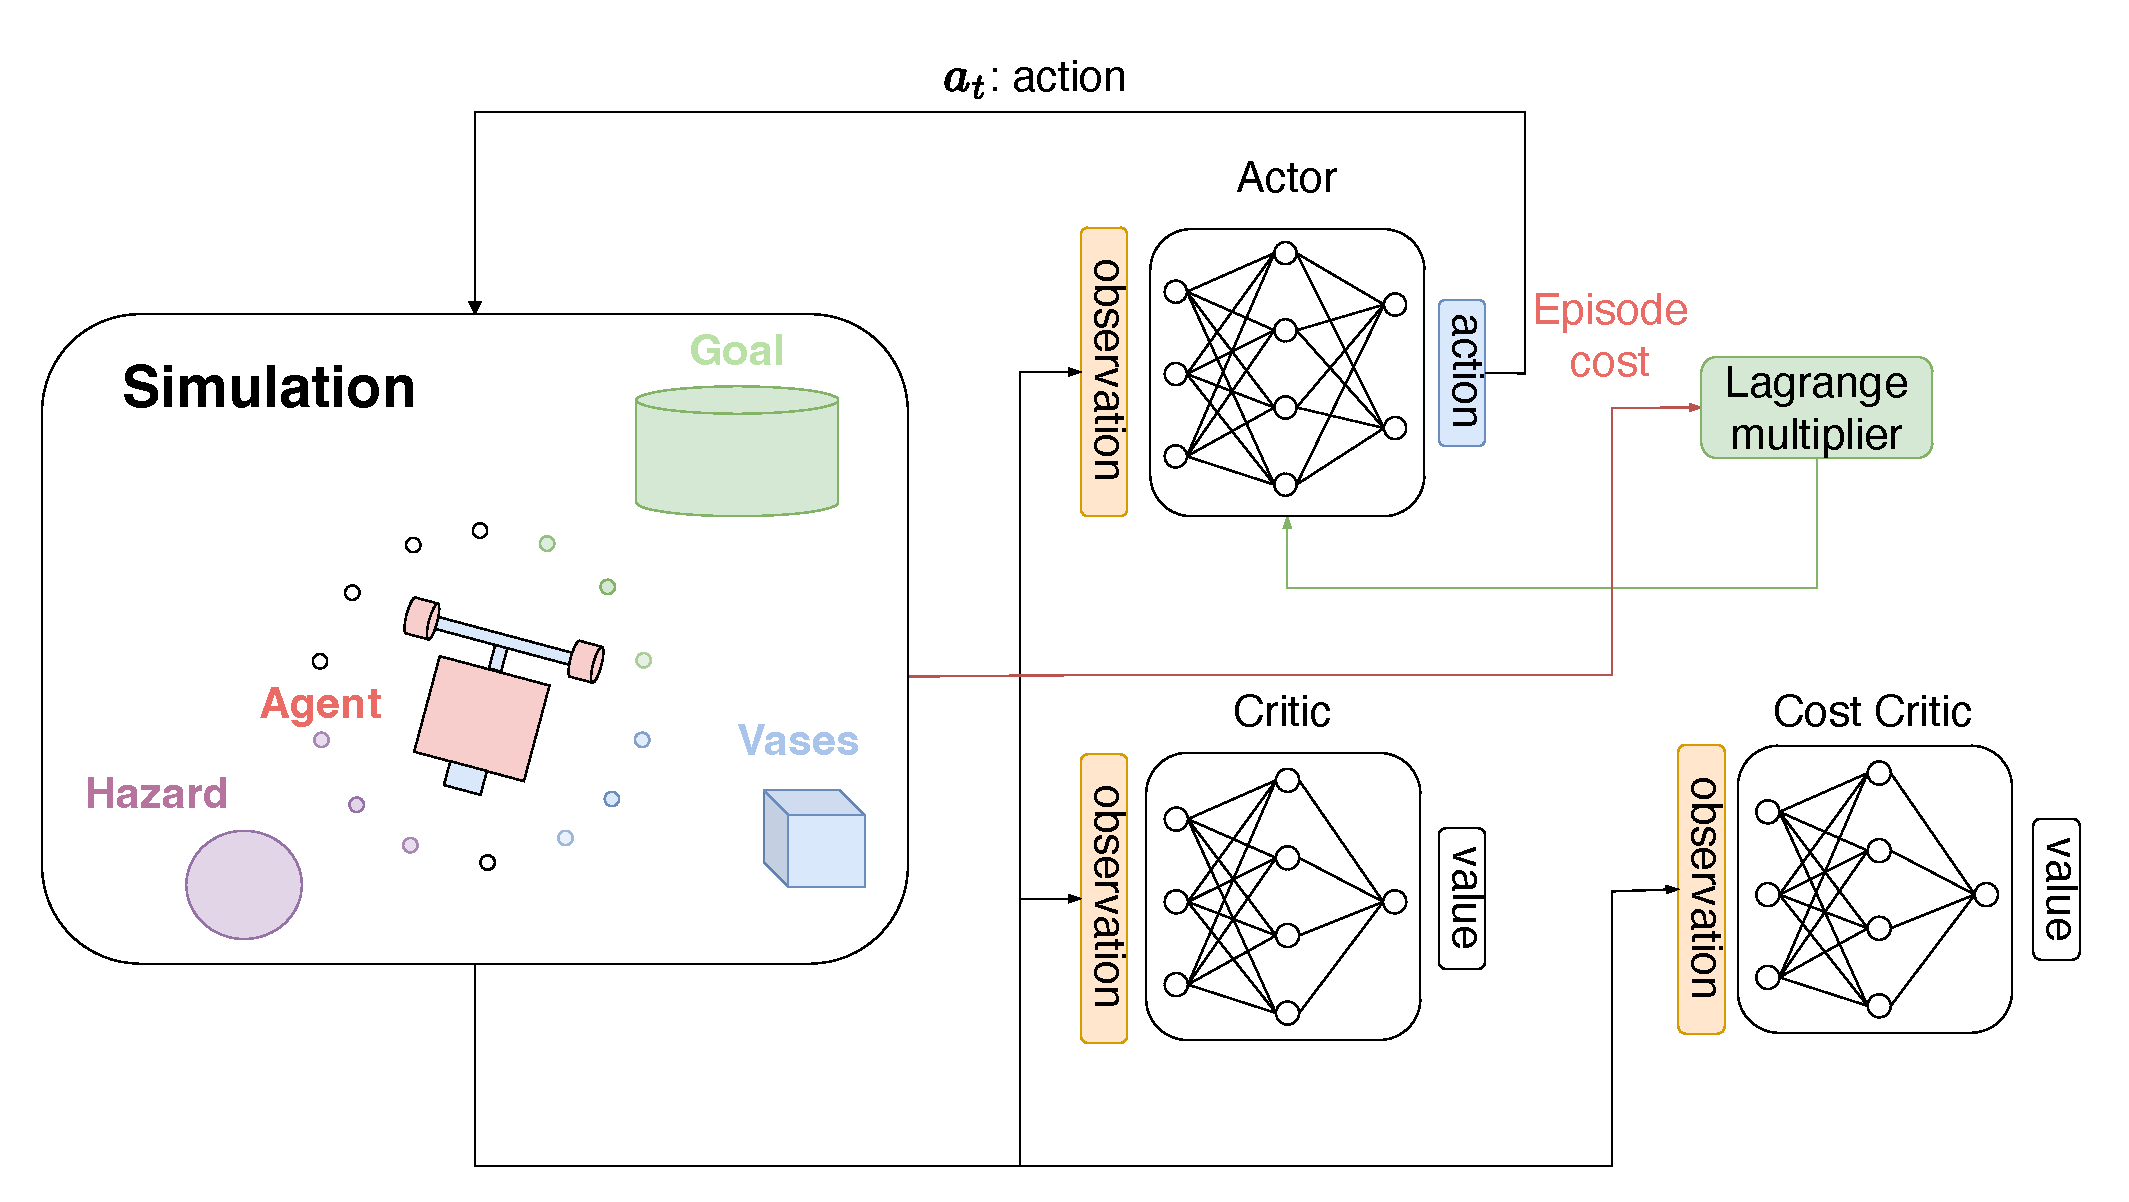
\includegraphics[width=1.0\textwidth]{imgs/chap2/ppo_lag.pdf}
  \caption{Structure of PPO Lagrangian}
  \label{chap2:fig:ppo_lag}
\end{figure*}

%%%%%%%%%%%%%%%%%%%%%%%%%%%%%%%%
\section{State-wise Constrained Reinforcement Learning} \label{chap2:sec5}
%%%%%%%%%%%%%%%%%%%%%%%%%%%%%%%%

State-wise Constrained Reinforcement Learning (SCRL) is a variant of CRL that imposes constraints at the state level.
CRL considers the cumulative cost over the entire trajectory, while SCRL focuses on the cost at each transition.
SCRL is formalized as a State-wise Constrained Markov Decision Process (SCMPD), it is quite similar to CMDP, but SCMDP enforces the constraint for every state action trasition satisfies a hard constraints.
The objective of SCRL is to find an optimal policy that maximizes the expected cumulative reward while satisfying the state-wise constraints.
\begin{equation}
  \begin{aligned}
    \pi^* &= \arg\max_{\pi_\theta} J(\theta) \\
    J(\theta) &= \mathbb{E}_{\tau \sim \pi_\theta} \left[ \sum^T_{t = 0} r_t \right] \; \text{subject to} \; \mathbb{E}_{\tau \sim \pi_\theta}  [c(s, a)] \leq w, \quad \forall s \in S
  \end{aligned}
\end{equation}

\subsection{Related Work: Feasible Actor-Critic} \label{chap2:sec5:fac}

Feasible Actor-Critic (FAC) is an extension of the Soft Actor-Critic algorithm to the SCRL setting \cite{FAC}.
In FAC, the state-wise constraint is enforced via a cost action-value function, formulated as:
\begin{equation}
  Q^{\pi_\theta}_c(s, a) = \mathbb{E}_{\tau \sim \pi_\theta}\left[\sum^T_{t = 0} c_t |s_0 = s, a_0 = ~a \right] \leq w
\end{equation}
The objective function of FAC is defined as:
\begin{equation} \label{chap2:eq:fac}
  \begin{aligned}
    J^{\text{FAC}}(\theta) = \mathbb{E}_{s_t \sim \mathcal{D}} \Big[ \mathbb{E}_{a_t \sim \pi_\theta} \big[ 
    &\alpha \log(\pi_\theta(a_t|s_t)) - Q_\phi(s_t, a_t) \\
    &+ \lambda_\xi(s_t)\left( Q_{\phi_c}(s_t, a_t) - w \right) 
    \big] \Big]
  \end{aligned}
\end{equation}
where $Q_{\phi_c}$ is the cost action-value function, and $\lambda_\xi$ is the Lagrange multiplier network, which estimate the Lagrange multiplier for each state.
The update of the Lagrange multiplier network depends on whether the cost action-value function exceeds the threshold $w$.
\begin{equation}
  J_\lambda(\xi) = \mathbb{E}_{s_t \sim \mathcal{D}} \left[ \mathbb{E}_{a_t \sim \pi_\theta} \left[ \lambda_\xi(s_t) \left( Q_{\phi_c}(s_t, a_t) - w \right) \right] \right]
\end{equation}
Fig.~\ref{chap2:fig:fac} illustrates the architecture of Feasible Actor-Critic (FAC). 
Since FAC is an off-policy algorithm, samples collected during the rollout phase are stored in a replay buffer, and mini-batches are drawn from it to update the actor, critics, and Lagrange multiplier network. 
The environment-provided reward and cost are used to update their respective Q-functions.
Using the reward and cost values estimated by the critic networks, together with the Lagrange multiplier computed from the Lagrange multiplier network, the policy is updated according to Equation~\ref{chap2:eq:fac}. 
The Lagrange multiplier network is updated based on the cost values estimated by the cost Q-function.
\begin{figure*}[h]
  \centering
  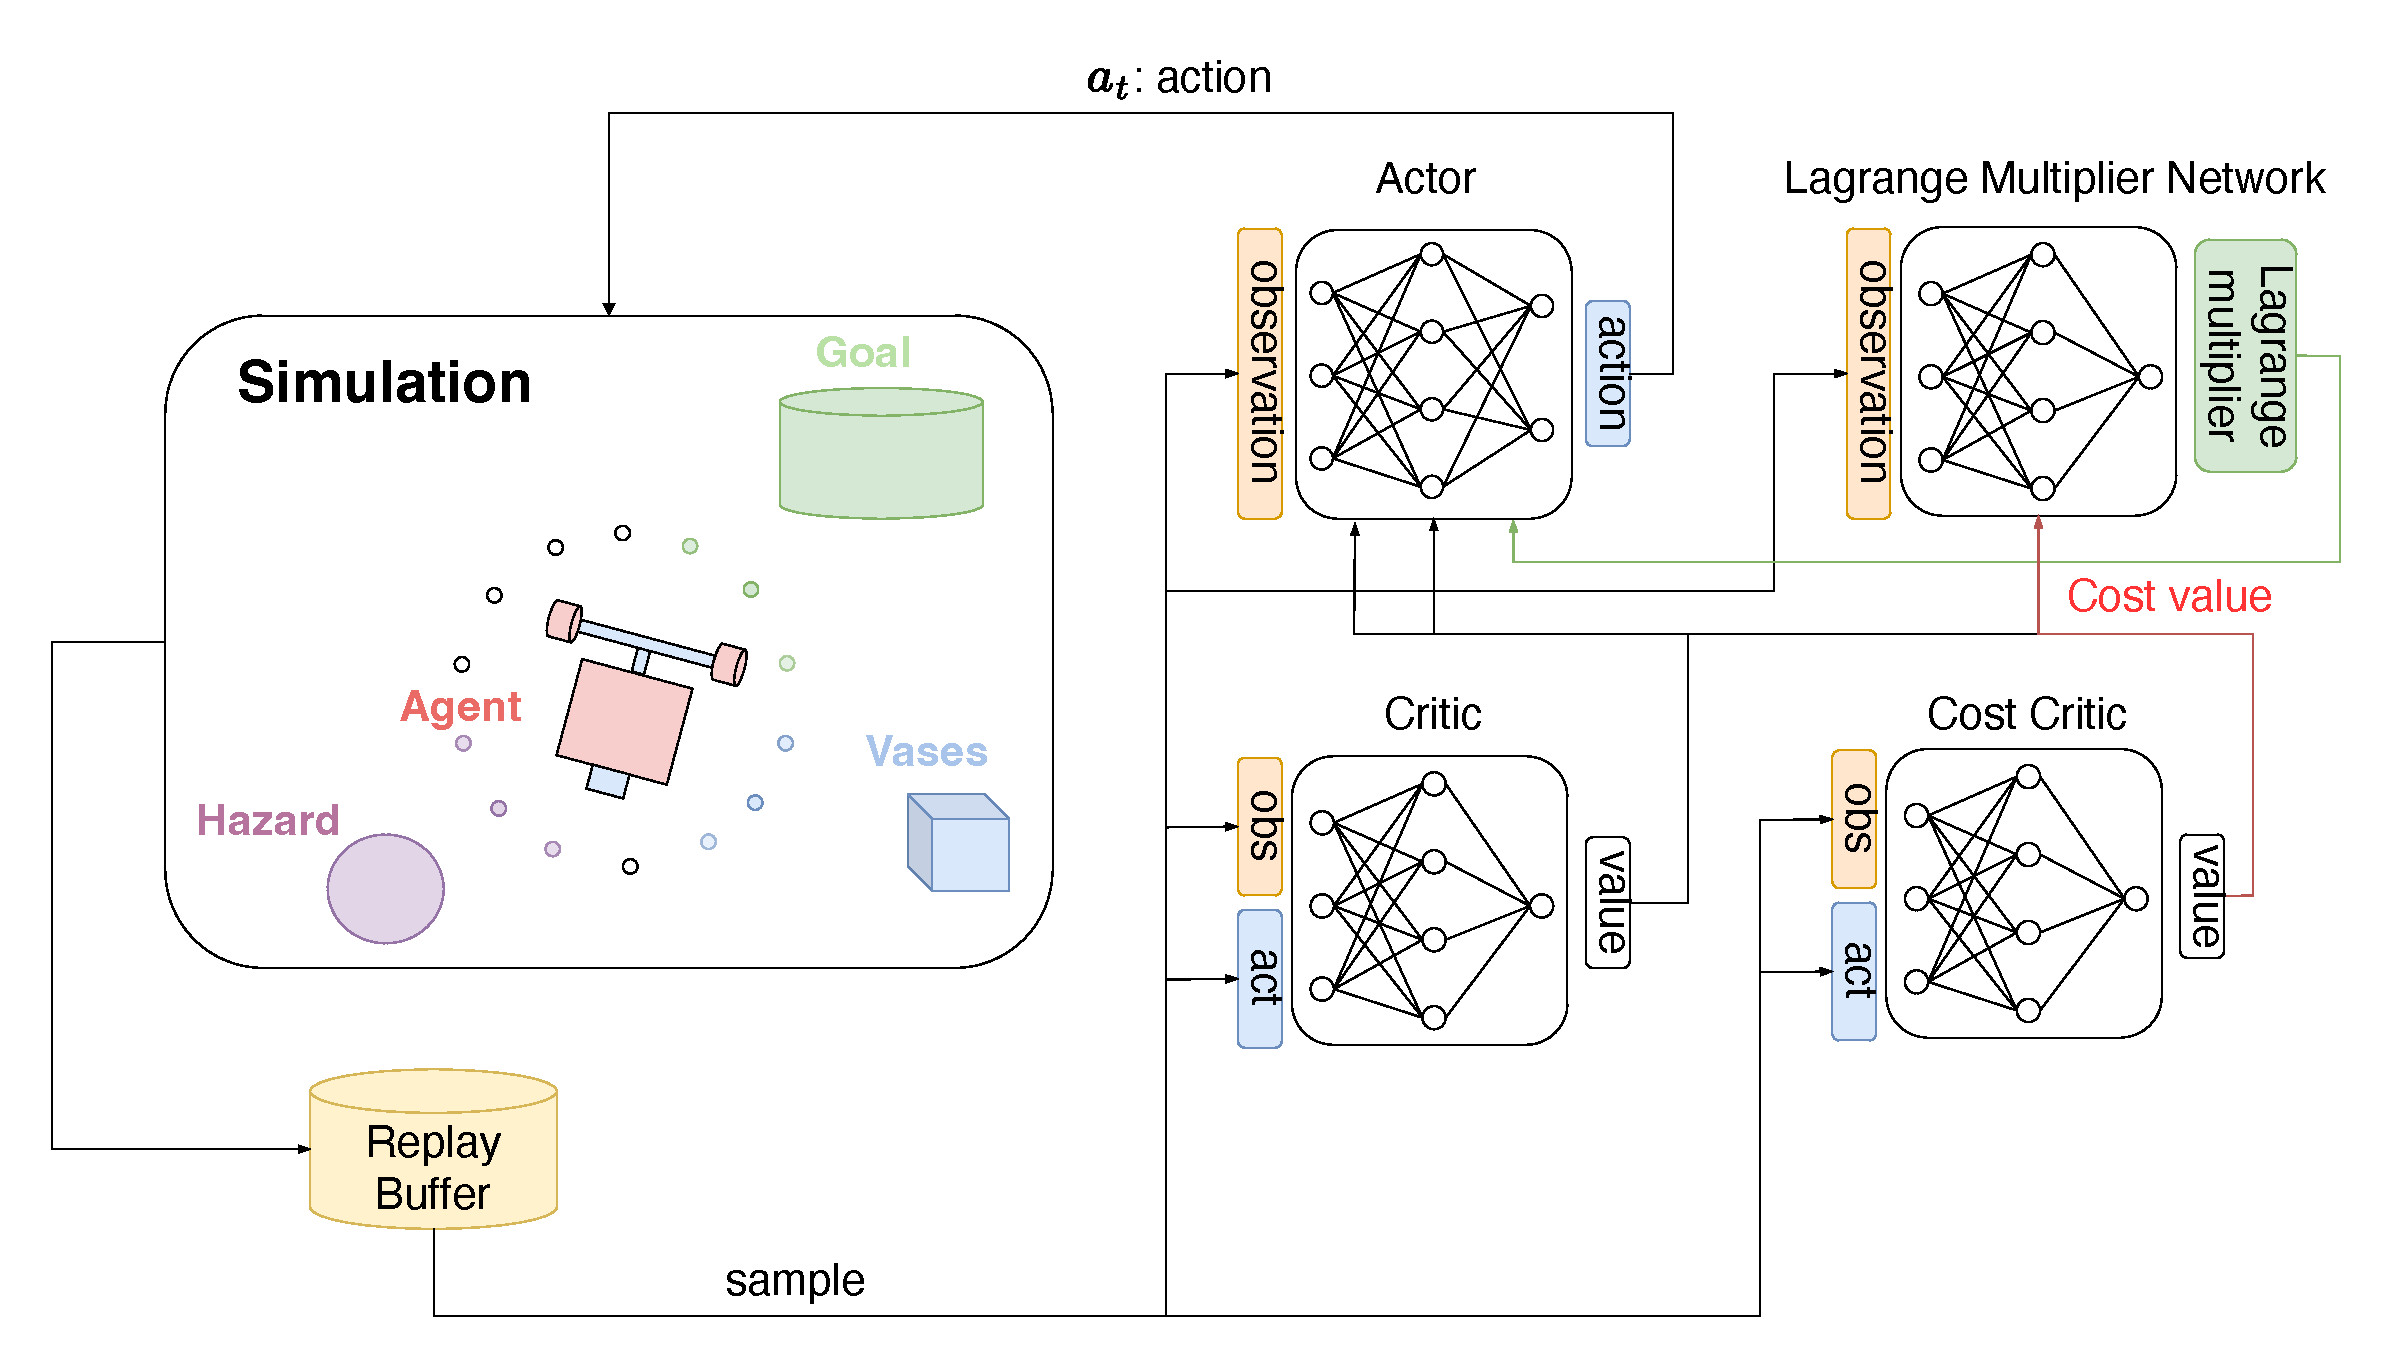
\includegraphics[width=1.0\textwidth]{imgs/chap2/fac.pdf}
  \caption{Structure of Feasible Actor-Critic}
  \label{chap2:fig:fac}
\end{figure*}

\noindent Although FAC contributes by proposing a framework that leverages a Lagrange multiplier network to address state-wise safety in policy learning, it has several limitations.
\begin{itemize}
  \item 
  Soft Actor-Critic (SAC) encourges exploration and promotes diverse action selection by adjusting the temperature parameter $\alpha$. 
  However, this objective can conflict with the constraint penalty term, which pushes the policy toward satisfying constraints. 
  As a result, it becomes more difficult for the policy consistently satisfy the constraints.
  \item 
  Instead of using the empirical cost values, FAC relies on a cost value estimated by the cost action-value function $Q_{\phi_c}(s, a)$.
  This introduces instability in the update of the Lagrange multiplier network due to potentially inaccurate cost estimates, which in turn can lead to unreliable policy updates.
\end{itemize}

\end{spacing}

%%%%%%%%%%%%%%%%%%%%%%%%%%%%%%%%%%%%
% Chapter 3 
%%%%%%%%%%%%%%%%%%%%%%%%%%%%%%%%%%%%

\begin{spacing}{2.0} % double spacing

%%%%%%%%%%%%%%%%%%%%%%%%%%%%%%%%
% Chap 3. PPO Lagrangian Network
%%%%%%%%%%%%%%%%%%%%%%%%%%%%%%%%

\chapter{PPO-based Method in State-wise Constrained RL}\label{chapter3}

\section{PPO Lagrangian Network}

As discussed in Section ~\ref{chap2:sec5:fac}, Feasible Actor-Critic (FAC) exhibits potential limitations arising from the characteristics of the SAC algorithm, its off-policy nature, and the way state-wise safety is defined through the cost Q-function.
In this chapter, we introduce our proposed method, which extends PPO under the state-wise constrained RL framework.
Similar to FAC method, we employ a network that estimates state-wise Lagrange multipliers to enforce safety constraints at the state level.
Thus, objective function of the policy is modified to include a Lagrange multiplier network:
% \begin{equation} \label{chap3:eq:ppo_lagnet}
%   J^{\text{PPO-Lagnet}}(\theta) = \mathbb{E}_{\pi_{\theta_\text{old}}} \left[ \min \left( r(\theta) A^{\pi_{\theta_\text{old}}}(s, a), \text{clip}(r(\theta), 1 - \epsilon, 1 + \epsilon)A^{\pi_{\theta_\text{old}}}(s, a) \right) - \lambda_\xi(s) r(\theta) A^{\pi_{\theta_\text{old}}}_c \right]
% \end{equation}
\begin{equation} \label{chap3:eq:ppo_lagnet}
  \begin{aligned}
    J^{\text{PPO-Lagnet}}(\theta) = \mathbb{E}_{\pi_{\theta_\text{old}}} \Big[ &\min \big( r(\theta) A^{\pi_{\theta_\text{old}}}(s, a), \text{clip}(r(\theta), 1 - \epsilon, 1 + \epsilon) A^{\pi_{\theta_\text{old}}}(s, a) \big) \\
    &- \lambda_\xi(s) r(\theta) A^{\pi_{\theta_\text{old}}}_c \Big]
  \end{aligned}
\end{equation}
where $A^{\pi_{\theta_\text{old}}}_c$ is the advantage function for the cost and $\lambda_\xi(s)$ is the Lagrange multiplier network that estimates the Lagrange multiplier for the cost at state $s$.
The Lagrange multiplier network is iteratively updated during training to guide the policy toward satisfying the imposed constraints.
The update of the Lagrange multiplier network depends on whether the empirical cost at state $s$ exceeds the threshold $w$:
\begin{equation}
  \lambda(s) \leftarrow \lambda(s) + \beta(\hat{J}_c - w)
\end{equation}
To ensure the positivity of the Lagrange multiplier, a softplus activation function is applied to the final layer of the network. 
\begin{figure*}[h]
  \centering
  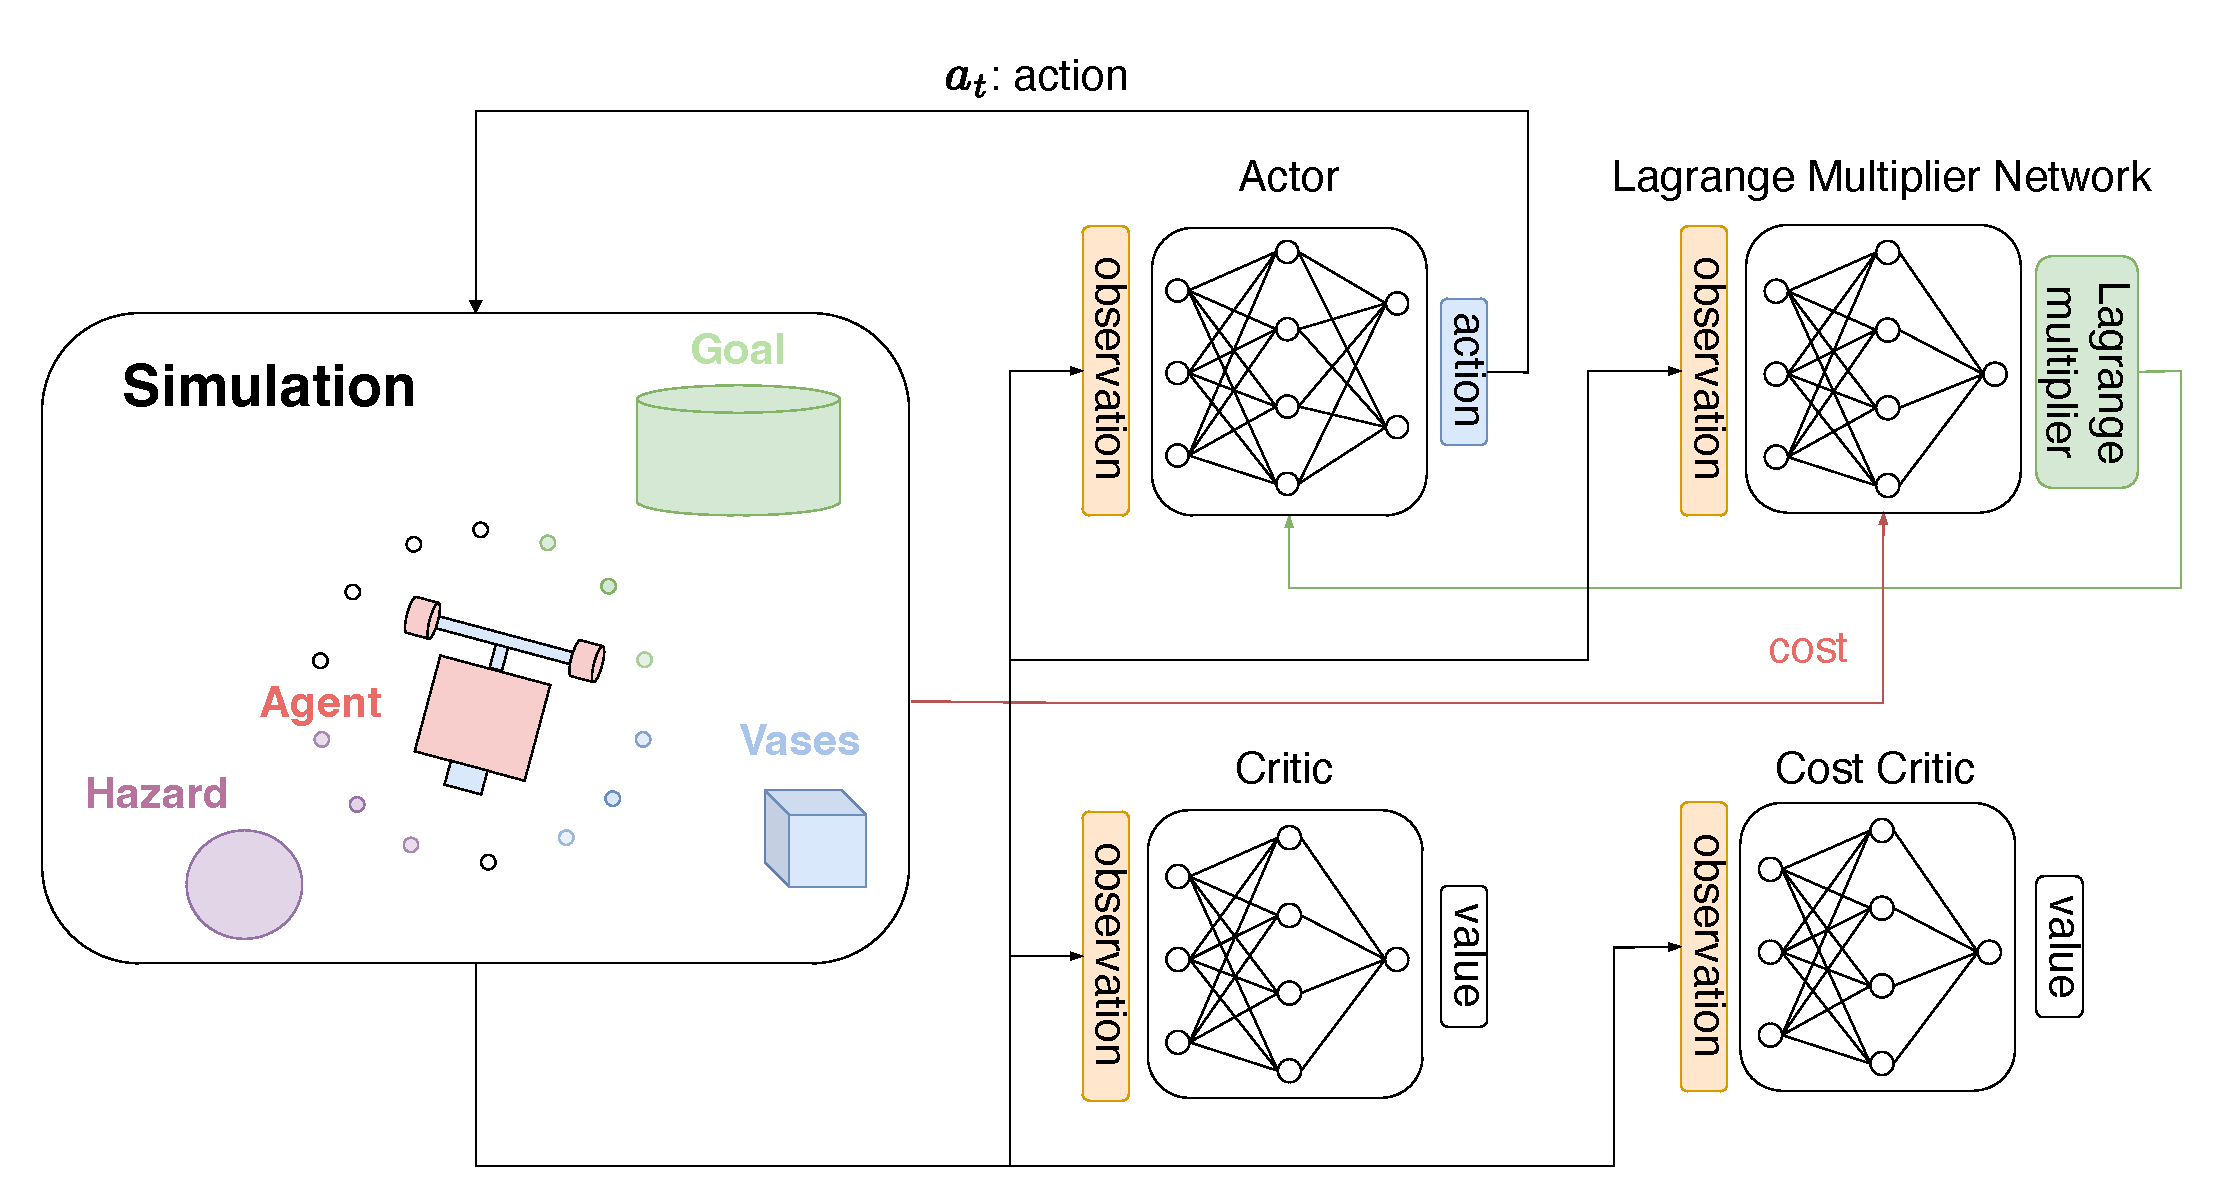
\includegraphics[width=1.0\textwidth]{imgs/chap3/ppo_lagnet.pdf}
  \caption{Structure of PPO Lagrangian Network}
  \label{chap3:fig:ppo_lagnet}
\end{figure*} \\
The overall architecture of the PPO Lagrangian Network is illustrated in Fig.~\ref{chap3:fig:ppo_lagnet}. 
The structure closely follows that of PPO Lagrangian described in Fig.~\ref{chap2:fig:ppo_lag}: 
the agent interacts with the environment using actions generated by the actor network, and the collected trajectories are used to estimate reward and cost returns at each state using the value function networks.
These return estimates are then used to compute the reward and cost advantages, which correspond to $A^{\pi_{\theta_\text{old}}}$ and $A^{\pi_{\theta_\text{old}}}_c$.
These advantages are then used to update the policy according to Equation~\ref{chap3:eq:ppo_lagnet}.
The key distinction from the PPO Lagrangian lies in the design of the Lagrange multiplier. 
Instead of using a single scalar multiplier, the PPO Lagrangian Network introduces a dedicated neural network that estimates a state-wise Lagrange multiplier $\lambda_\xi(s)$, which is updated based on the cost incurred at each individual state within the trajectories.
This allows the algorithm to enforce constraints more precisely at the state level rather than relying on trajectory-level cost.

\begin{algorithm}
  \DontPrintSemicolon
  \caption{PPO Lagrangian Network}
  \KwIn{Initial policy parameters $\theta_0$, initial value function parameters $\phi_0$, initial cost value function parameters $\phi^c_0$, Lagrange multiplier network parameters $\xi$, threshold $w$}
  \For{each epoch $k = 0, 1, 2, \cdots$}{
    \For{each time step $t = 1$ \KwTo $T$}{
      \tcp{Collect trajectories}
      Sample action $a_t \sim \pi_{\theta_{t - 1}}(s_t)$ \;
      Execute action $a_t$ in the environment and observe reward $r_t$, cost $c_t$ and next state $s_{t + 1}$ \;
      Store transition $\tau_t = (s_t, a_t, r_t, c_t, s_{t+1})$ in buffer $D_k$ \;

      \If{episode end}{
        Compute rewards-to-go $\hat{R}_t$ and advantage estimates $\hat{A}_t$ based on the current value function $V_{\phi_k}$ \;
        Compute costs-to-go $\hat{R}^c_t$ and cost advantage estimates $\hat{A}^c_t$ based on the current cost value function $V^c_{\phi_k}$ \;
      }
    }
    \BlankLine
    
    \tcp{Lagrange multiplier network update}
    Update the Lagrange multiplier $\lambda$ by gradient ascent:
    \begin{equation*}
        \xi_{k + 1} = \xi_k + \beta \left[ \frac{1}{|D_k|T} \sum_{\tau \in D_k} \sum^T_{t = 0} (c_t - w) \right]
    \end{equation*}
    \BlankLine

    \tcp{Policy update}
    Update the policy parameters $\theta$ by maximizing the objective function:
    \begin{equation*}
      \begin{aligned}
        \theta_{k + 1} = \arg \max \frac{1}{|D_k|T} \sum_{\tau \in D_k} \sum^T_{t = 0} \Big[ &\min \left( r_t(\theta) \hat{A}^{\pi_{\theta_k}}(s_t, a_t), \; g\left( \epsilon, \hat{A}^{\pi_{\theta_k}}(s_t, a_t) \right) \right) \\
        & - \lambda_\xi (s_t) r_t(\theta) \hat{A}^{\pi_{\theta_k}}_c (s_t, a_t)  \Big]\\
        \text{where }
        r_t(\theta) = \frac{\pi_\theta(a_t|s_t)}{\pi_{\theta_k}(a_t|s_t)}, \;
        &g(\epsilon, A) = 
          \begin{cases}
            (1 + \epsilon)A \quad A \geq 0 \\
            (1 - \epsilon)A \quad A < 0
          \end{cases}
      \end{aligned}
    \end{equation*}    
    \BlankLine

    \tcp{Value function update}
    Fit value function by regression on mean-squared error:
    \begin{equation*}
      \begin{aligned}
        \phi_{k + 1} &= \arg\min_\phi \frac{1}{|D_k|T} \sum_{\tau \in D_k} \sum^T_{t = 0} \left( V_\phi(s_t) - \hat{R}_t \right)^2 \\
        \phi^c_{k + 1} &= \arg\min_\phi \frac{1}{|D_k|T} \sum_{\tau \in D_k} \sum^T_{t = 0} \left( V_{\phi^c}(s_t) - \hat{R}^c_t \right)^2
      \end{aligned}
    \end{equation*}
    % typically via stochastic gradient descent algorithm.
  }
\end{algorithm}

\subsection{Comparison with PPO Lagrangian}

In PPO Lagrangian, the Lagrange multiplier is a scalar because it enforces that the cumulative cost along trajectories generated by the policy $\pi_\theta$ remains below a specified threshold.
In contrast, PPO Lagrangian Network estimates a state-wise Lagrange multiplier, which enables the policy to satisfy cost constraints more precisely at each individual state by enforcing the cost at each state to remain below the specified threshold.

\subsection{Comparison with Feasible Actor-Critic}

Feasible Actor-Critic (FAC) is similar to PPO Lagrangian Network in that it also estimates a state-wise Lagrange multiplier.
However, unlike FAC, our method updates the Lagrange multiplier network in a different way.
In FAC, the update is based on the output of the cost action-value network, which estimates the state-wise cost value.
In contrast, our proposed method updates the policy based on the actual cost values observed for each state.

\end{spacing}

%%%%%%%%%%%%%%%%%%%%%%%%%%%%%%%%%%%%
% Chapter 4
%%%%%%%%%%%%%%%%%%%%%%%%%%%%%%%%%%%%

\begin{spacing}{2.0} % double spacing
  
%%%%%%%%%%%%%%%%%%%%%%%%%%%%%%%%
% Chap 4. Experiments
%%%%%%%%%%%%%%%%%%%%%%%%%%%%%%%%

\chapter{Experiments}\label{chapter4}

\section{Setup} \label{chap4:sec:setup}

For our experiments, we use the OpenAI Safety Gym \cite{PPO-Lagrangian, Safety-Gymnasium} environments.
OpenAI no longer maintains Safety Gym, and its development has been continued since 2023 by the PKU-Alignment Team under the name Safety Gymnasium.
Safety Gymnasium preserves full compatibility with the original Safety Gym environments, including identical reward functions, cost functions, agents, and other components.
To avoid confusion, we refer to these environments as Safety Gym throughout this thesis.
In Safety Gym environements, there are three types of agents: Point, Car, and Doggo.
In our experiments, we use the Car agent provided in Safety Gym.
\begin{itemize}
    % \item \textbf{Point}: A simple 2D robot with two actuators—one for turning and another for forward/backward motion. The Point agent appears on the far left in Fig.~\ref{chap4:fig:cost}.
    \item \textbf{Car}: A car-like robot with two independently controlled front wheels and a passive rear wheel. Since both forward movement and turning must be controlled together, it is slightly more difficult to operate than the Point. The Car agent is shown in Fig.~\ref{chap4:fig:reward}.
\end{itemize}
Also, there are three types of tasks: Goal, Button, and Push.
We use two of the tasks provided in Safety Gym: Goal and Button.
\begin{itemize}
    \item \textbf{Goal}: The agent must reach a goal location while avoiding obstacles.
    \item \textbf{Button}: The agent must press a button while avoiding obstacles.
    \item \textbf{Push}: The agent must push yellow box to a goal location while avoiding obstacles.
\end{itemize}
The reward function provides positive rewards as the agent moves closer to the goal, and negative rewards as it moves farther away:
$ r_t = d_{t - 1} - d_t $, where $d_t$ is the distance to the goal at time $t$.
Additionally, each task provides an extra positive reward when the agent successfully completes the objective, such as reaching the goal, pressing a button, or moving a box.
\begin{figure*}[h]
  \centering
  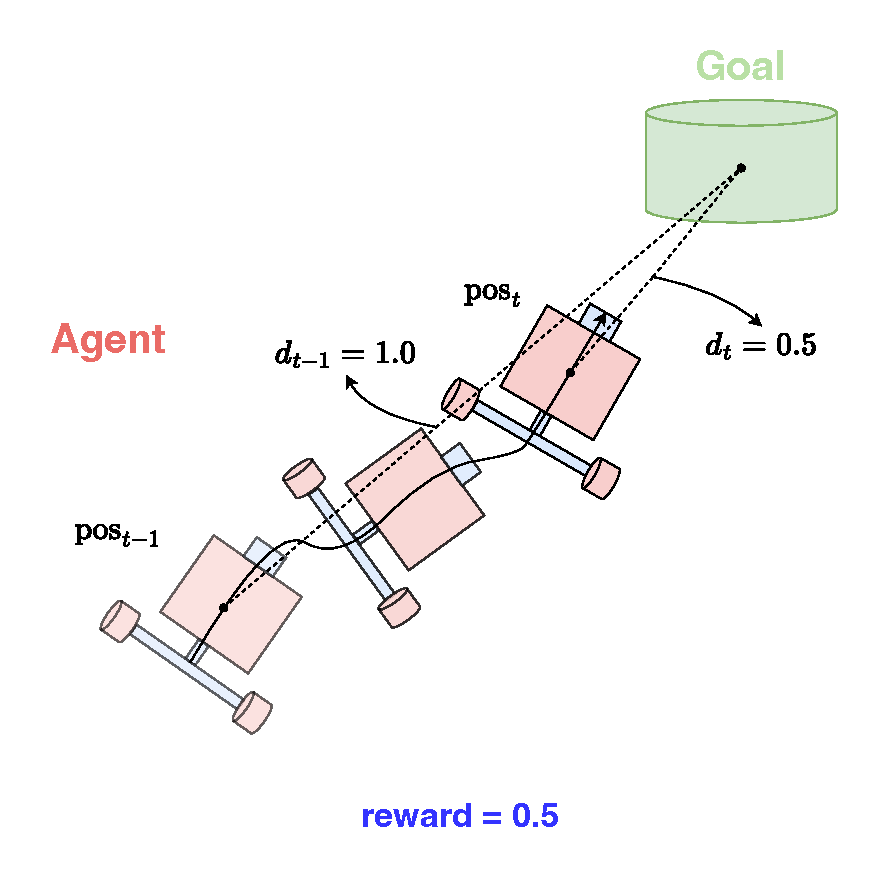
\includegraphics[width=0.5\textwidth]{imgs/chap4/setup/reward.pdf}
  \caption{Illustration of how reward is computed in the Safety Gym}
  \label{chap4:fig:reward}
\end{figure*}

\begin{figure*}[h]
  \centering
  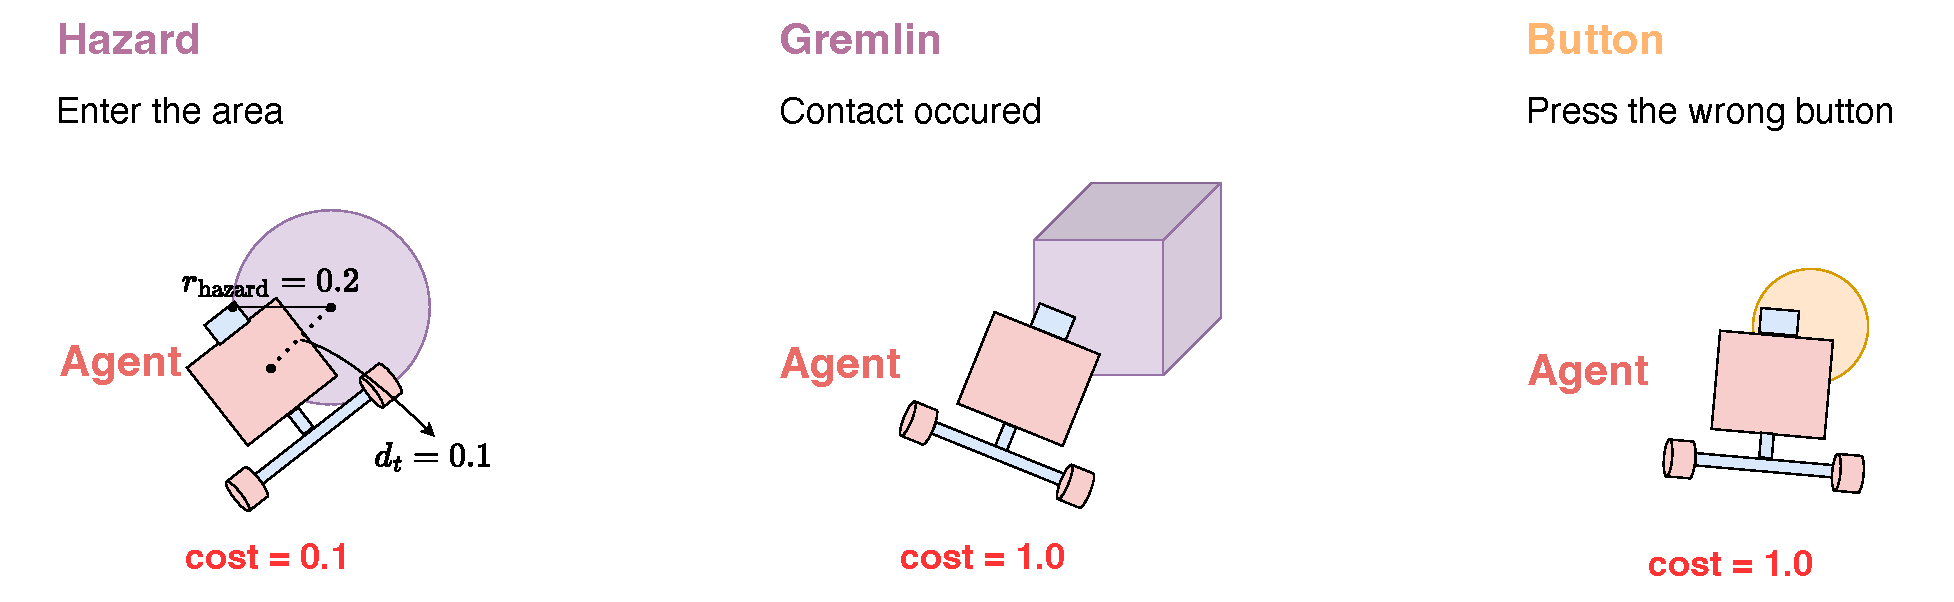
\includegraphics[width=1.0\textwidth]{imgs/chap4/setup/cost.pdf}
  \caption{Illustration of how costs are computed in the Safety Gym}
  \label{chap4:fig:cost}
\end{figure*}

The cost function varies depending on the types of obstacles present in each task.
In our experimental environments, three types of obstacles are used, as illustrated in Fig.~\ref{chap4:fig:cost}:
\begin{itemize}
    \item \textbf{Hazard}: A cost is assigned when the agent enters a hazard area. The cost is computed as $c_t = d_t - r_{\text{hazard}}$, where $d_t$ is the distance from the agent to the center of the hazard and $r_{\text{hazard}} = 0.2$ is the hazard radius.
    \item \textbf{Gremlin}: A cost of $-1.0$ is incurred when the agent makes contact with the gremlin object.
    \item \textbf{Button}: A cost of $-1.0$ is assigned when the agent presses a button that is not the designated goal button.
\end{itemize}
A key distinction of this thesis compared to other works lies in how the cost function is defined.
Safety Gym provides two options for computing cost: a dense formulation and a sparse (indicator) cost.
Many prior works adopt the sparse cost, where the environment returns 1 if a cost-triggering event occurs and 0 otherwise.
In contrast, this thesis uses the dense cost described above, where the cost value is computed at each time step based on factors such as distance to obstacles or safety-related conditions.
This choice is motivated by the fact that using sparse costs makes it difficult to precisely define and enforce constraint conditions.
Dense costs allow for more precise and informative constraint definitions compared to sparse costs.

%%%%%%%%%%%%%%%%%%%%%%%%%%%%%%%%
\section{Analyzing the Influence of alpha in the Feasible Actor-Critic} \label{chap4:sec:experiments:fac}
%%%%%%%%%%%%%%%%%%%%%%%%%%%%%%%%

As discussed in Section~\ref{chap2:sec3:sac}, Soft Actor-Critic (SAC) promotes stochastic exploration by maximizing both expected return and policy entropy. 
The temperature parameter $\alpha$ controls the importance of the entropy term: larger values of $\alpha$ encourage more exploratory and diverse action selection.
However, in the Feasible Actor-Critic (FAC) framework, this exploration objective can conflict with the effect of the Lagrange multiplier, which encourages the policy to satisfy safety constraints.
To examine this trade-off, we compare the training performance of unconstrained SAC (yellow curve) and FAC with various fixed $\alpha$ values, using Fig.~\ref{chap4:fig:fac_return}, Fig.~\ref{chap4:fig:fac_cost}.
In Figure~\ref{chap4:fig:fac_cost}, although small spikes are present, FAC with all tested $\alpha$ values generally maintains a lower cost compared to unconstrained SAC.
This indicates that the constraint-satisfying mechanism in FAC is working as designed, leading to lower cost return by enforcing state-wise constraints more effectively.
On the other hand, the return curves in Figure~\ref{chap4:fig:fac_return} reveal that with $\alpha = 0.001$ (green), the return improves rapidly in the early phase (up to around 200 epochs), but then gradually declines and converges toward zero.
This behavior suggests that when $\alpha$ is relatively large, the entropy term dominates the learning signal, making the policy overly stochastic and less sensitive to both reward and constraint signals—ultimately degrading policy performance.
Based on these observations, we fix $\alpha$ to a small value of $0.00001$ for all subsequent comparisons between FAC and our proposed method, to minimize the entropy-induced instability while retaining some degree of exploration.

\begin{figure*}[h]
  \centering
  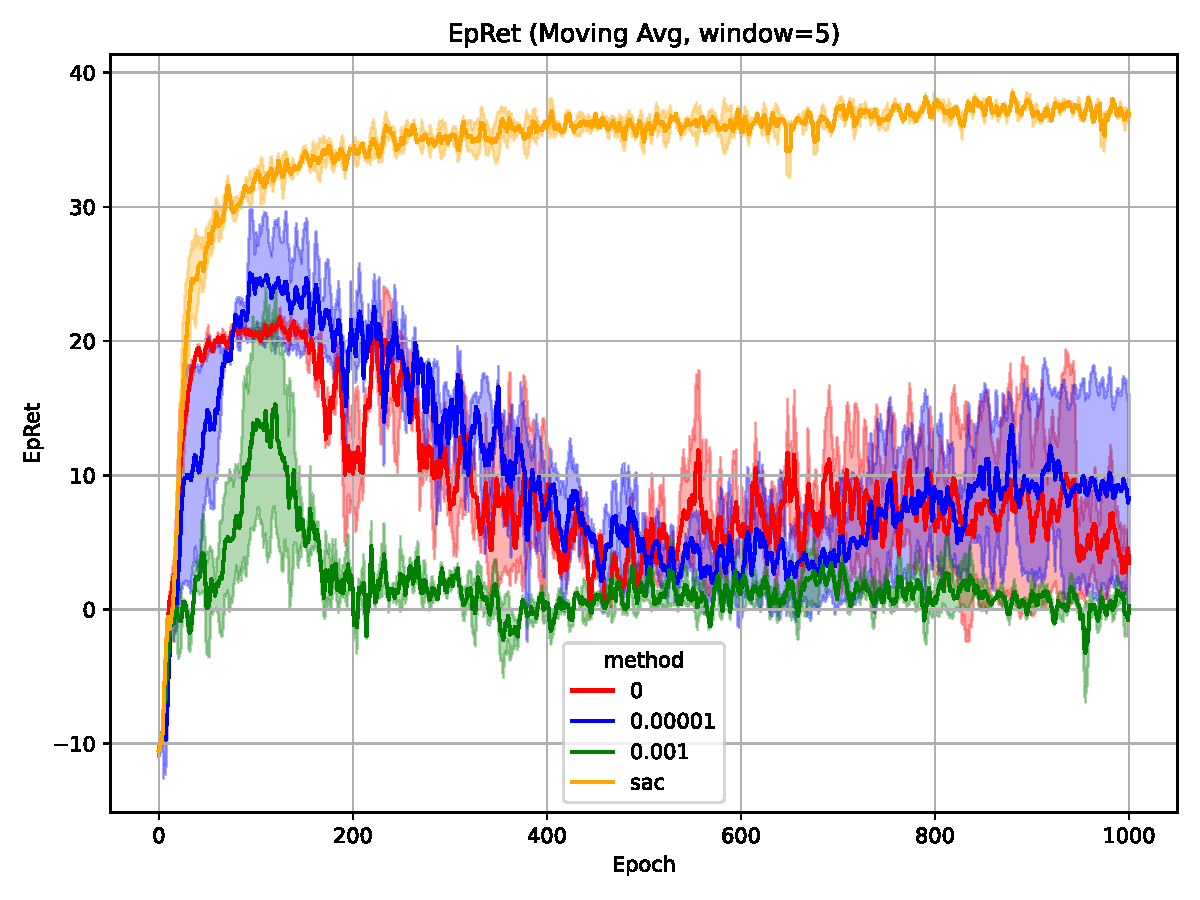
\includegraphics[width=0.65\textwidth]{imgs/chap4/fac/return.pdf}
  \caption{Training curves of return over epochs for different temperature parameters $\alpha$ in the Feasible Actor-Critic algorithm}
  \label{chap4:fig:fac_return}
\end{figure*}

\begin{figure*}[h]
  \centering
  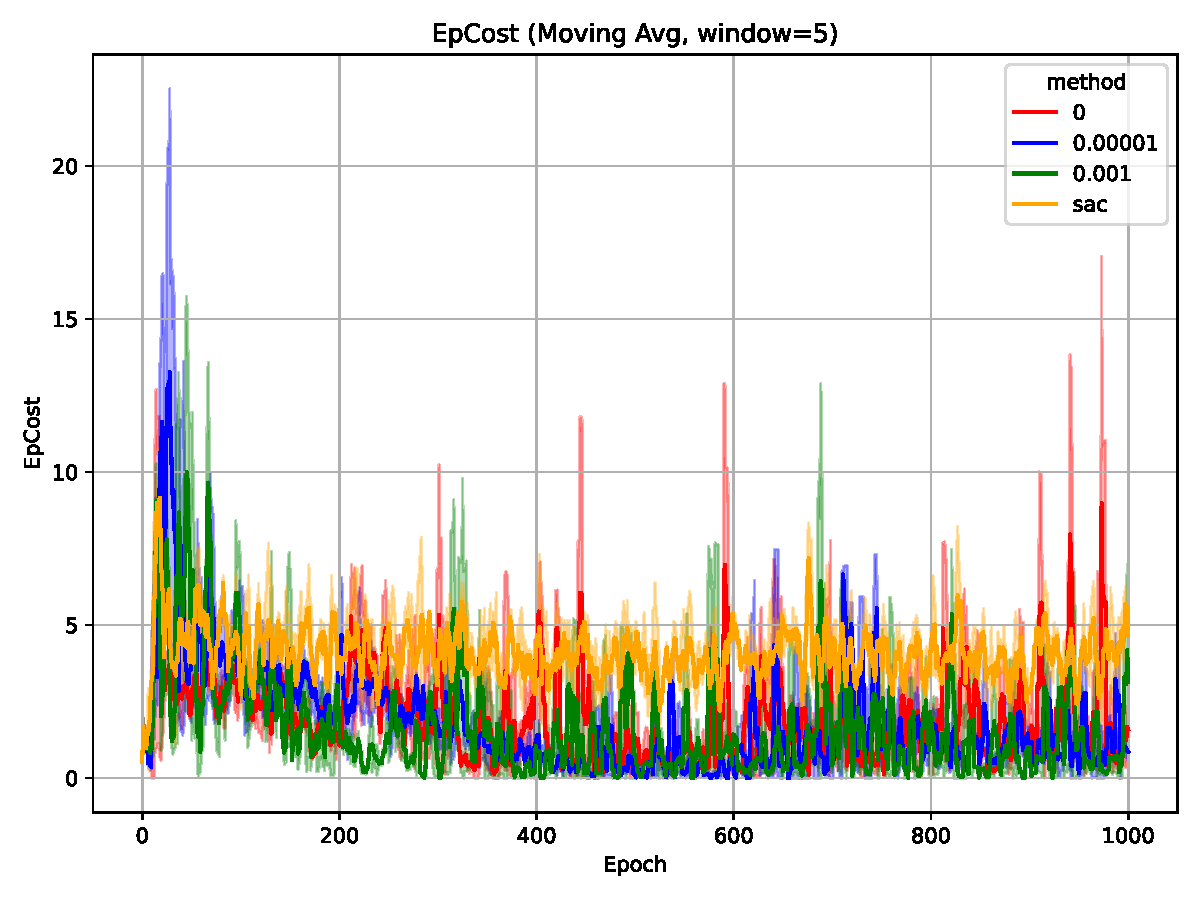
\includegraphics[width=0.65\textwidth]{imgs/chap4/fac/cost.pdf}
  \caption{Training curves of cost return over epochs for different temperature parameters $\alpha$ in the Feasible Actor-Critic algorithm}
  \label{chap4:fig:fac_cost}
\end{figure*}

\clearpage

\begin{table}[h]
  \centering
  \caption{Hyperparameters used in Experiment \ref{chap4:sec:experiments:fac}}
  \label{tab:hyperparams-fac}
  \begin{tabular}{l c}
    \toprule
    \textbf{Hyperparameter} & \textbf{Value} \\
    \midrule
    Environment                         & Car Goal \\
    Number of epochs                    & 1000 \\
    Number of steps per epoch           & 2000 \\
    Batch size                          & 256 \\
    Hidden layer size (MLP)             & 256 \\
    gamma (discount factor)             & 0.99 \\
    polyak (target network update)      & 0.995 \\
    Learning rate (policy)              & 5e-6 \\
    Learning rate (value function)      & 1e-3 \\
    Learning rate (Lagrange multiplier) & 5e-8 \\
    Lagrange multiplier init (bias)     & 0 \\    
    \bottomrule
  \end{tabular}
\end{table}

%%%%%%%%%%%%%%%%%%%%%%%%%%%%%%%%
\section{Analyzing the Influence of Bias Initialization in the Lagrange Multiplier Network of PPO Lagrangian Network} \label{chap4:sec:experiments:lagrange_init}
%%%%%%%%%%%%%%%%%%%%%%%%%%%%%%%%

Lagrangian-based methods are known to be sensitive to both initialization and learning rate \cite{CRL-survey}. 
Improper initialization of the Lagrange multiplier network can lead to suboptimal or delayed policy convergence. 
In particular, a large initial value may overly penalize the policy, driving it prematurely toward a local optimum, while a small initial value may result in slow adaptation of the constraint enforcement.
To analyze the effect of bias initialization,  we conducted experiments by varying the initial bias value of the final layer in the Lagrange multiplier network. 
Specifically, we manually initialized the bias term of the last linear layer to one of four values: 0, 20, 40, and 60.

\begin{figure*}[h]
  \centering
  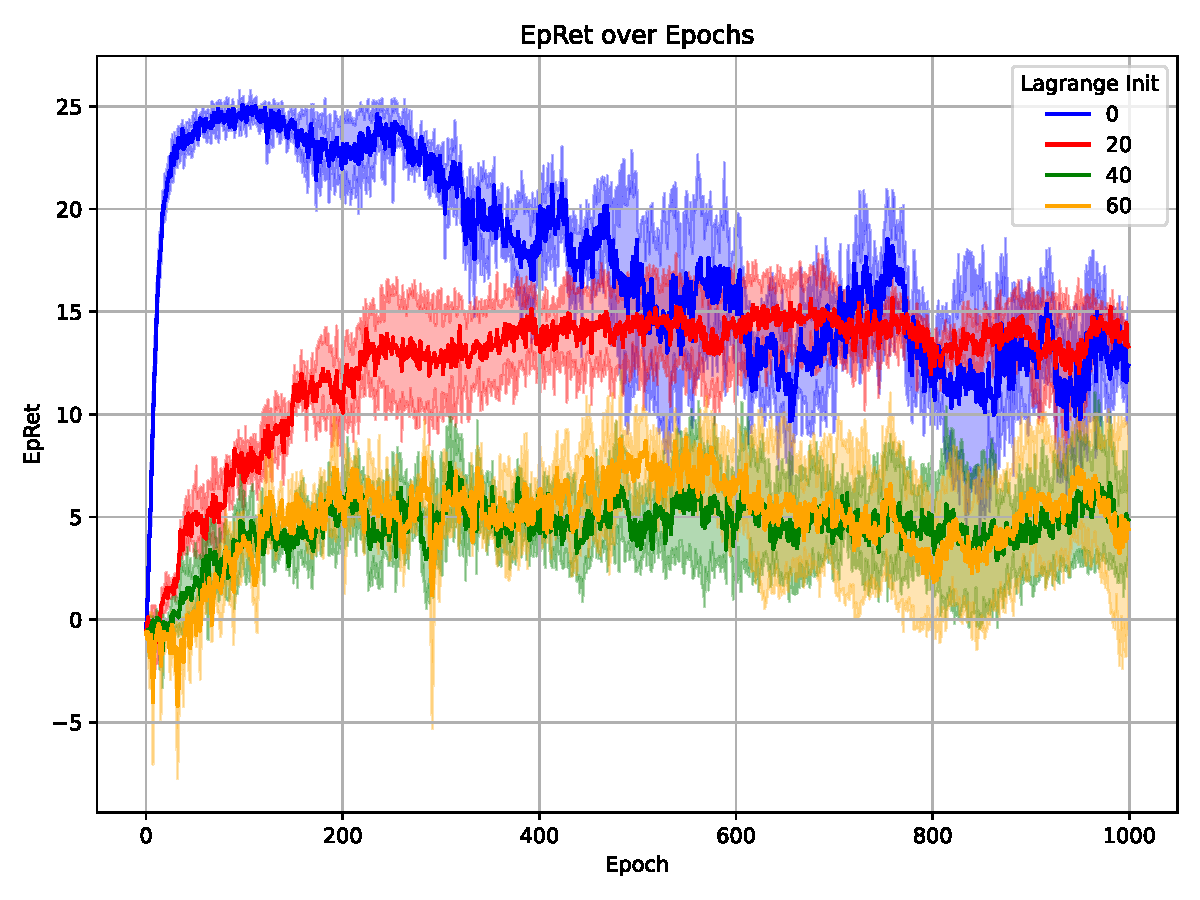
\includegraphics[width=0.65\textwidth]{imgs/chap4/lagrange_init/return.pdf}
  \caption{Training curves of return over epochs for different bias initializations in the Lagrange multiplier network}
  \label{chap4:fig:lagrange_init_return}
\end{figure*}

In Fig.~\ref{chap4:fig:lagrange_init_return}, shows the training curves of return over 1000 epochs for different bias initializations of the Lagrange multiplier network.
Although the convergence behavior varies across initial values, all four settings demonstrate stable policy learning overall.
When the initial bias is set to 0, the early phase (epoch $0 \sim 300$) closely resembles unconstrained PPO, showing a rapid increase in return.
However, as the Lagrange multiplier values grow, the return gradually decreases, indicating stronger constraint enforcement over time.
With an initial bias of 20, the agent achieves the most stable and effective learning performance, maintaining high return while satisfying constraints.
In contrast, higher initializations (40 and 60) result in excessive penalty signals, which overly constrain the policy.
This leads to premature convergence to suboptimal solutions, likely due to limited exploration or overly conservative policy updates.

\begin{figure*}[h]
  \centering
  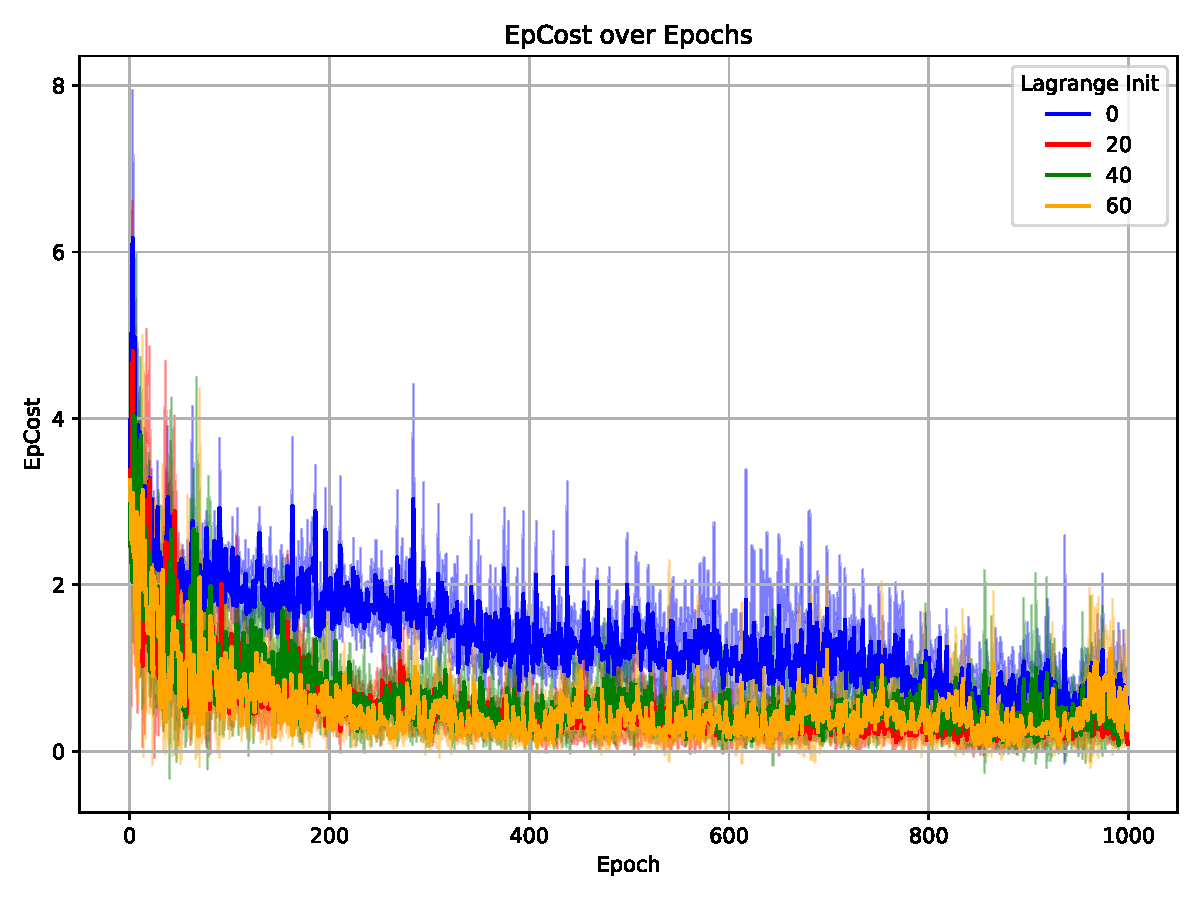
\includegraphics[width=0.65\textwidth]{imgs/chap4/lagrange_init/cost.pdf}
  \caption{Training curves of cost return over epochs for different bias initializations in the Lagrange multiplier network}
  \label{chap4:fig:lagrange_init_cost}
\end{figure*}

As shown in Fig.~\ref{chap4:fig:lagrange_init_cost}, all four settings demonstrate a stable reduction in cost over the course of training.
This indicates that the Lagrange multiplier network, regardless of initialization, is able to learn to enforce constraints effectively.
However, when comparing the results more closely, we observe that the setting with an initial bias of 0 achieves less cost reduction compared to the setting with an initial bias of 20, despite both eventually reaching similar Lagrange multiplier values (see Fig.~\ref{chap4:fig:lagrange_init_lagrange}). 
This suggests that early enforcement of constraints plays an important role in guiding the policy to safer regions of the state space.
In the zero-initialization case, the Lagrange multiplier grows more slowly, allowing higher constraint violations in the early phase of training.
As a result, the policy may have already been shaped in a way that is less sensitive to cost signals, making later enforcement of constraints less effective and leading to suboptimal cost minimization.
Therefore, initializing the Lagrange multiplier with a moderately large value (e.g., 20) helps stabilize training by better balancing the trade-off between reward and cost throughout learning.

\begin{figure*}[h]
  \centering
  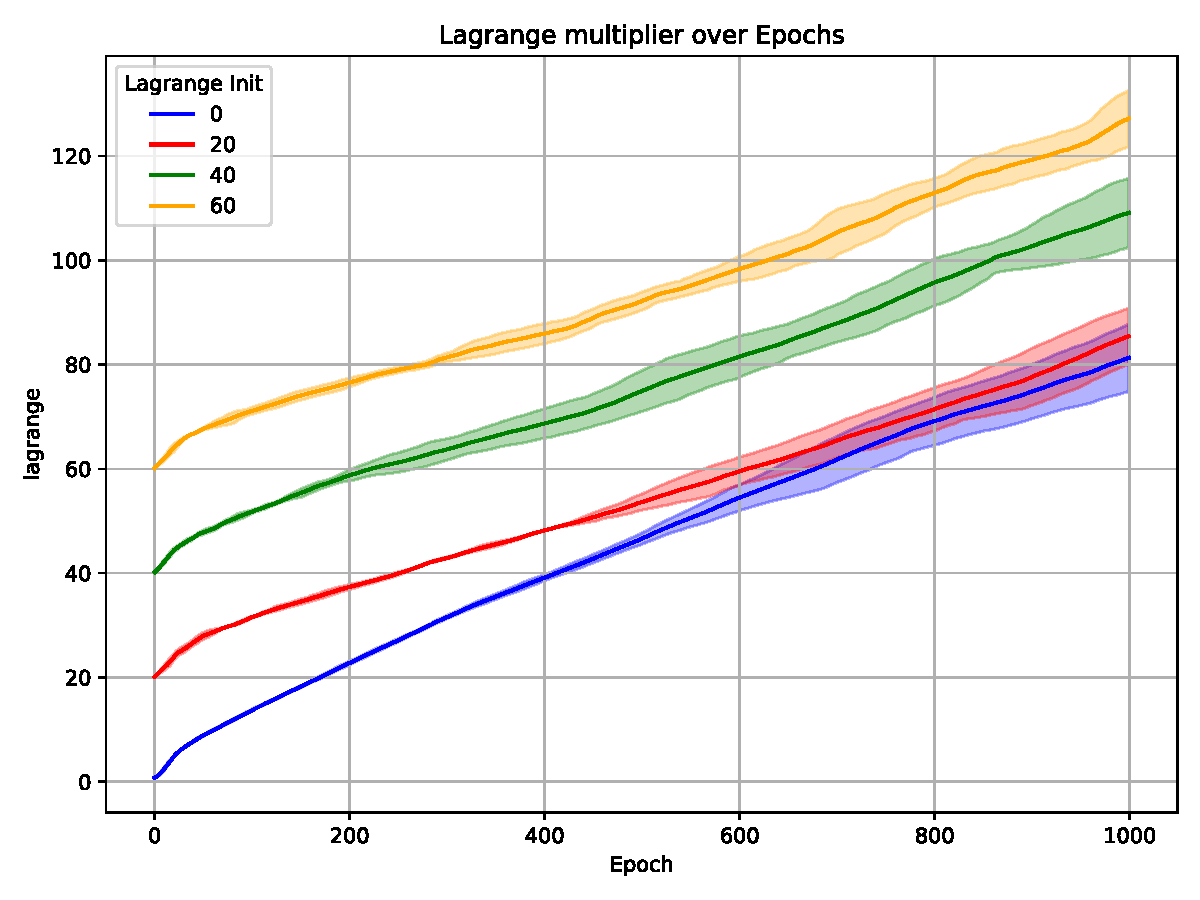
\includegraphics[width=0.65\textwidth]{imgs/chap4/lagrange_init/lagrange.pdf}
  \caption{Training curves of Lagragne multiplier over epochs for different bias initializations in the Lagrange multiplier network}
  \label{chap4:fig:lagrange_init_lagrange}
\end{figure*}

%%%%%%%%%%%%%%%%%%%%%%%%%%%%%%%%
\section{Analyzing the Influence of Learning Rate in the Lagrange Multiplier Network of PPO Lagrangian Network} \label{chap4:sec:experiments:lagrange_lr}
%%%%%%%%%%%%%%%%%%%%%%%%%%%%%%%%

The learning rate of the Lagrange multiplier network also plays a crucial role in stability and convergence. 
If the learning rate is too high, the multiplier may oscillate excessively, causing unstable policy updates. 
Conversely, if it’s too low, the multiplier may adapt too slowly to apply appropriate penalties.
To analyze the effect of the learning rate in the Lagrange multiplier network, we conducted experiments by varying the learning rate used for optimizing the network parameters.
Specifically, we tested three different learning rate values: 0.0003, 0.003, and 0.03.

\begin{figure*}[h]
  \centering
  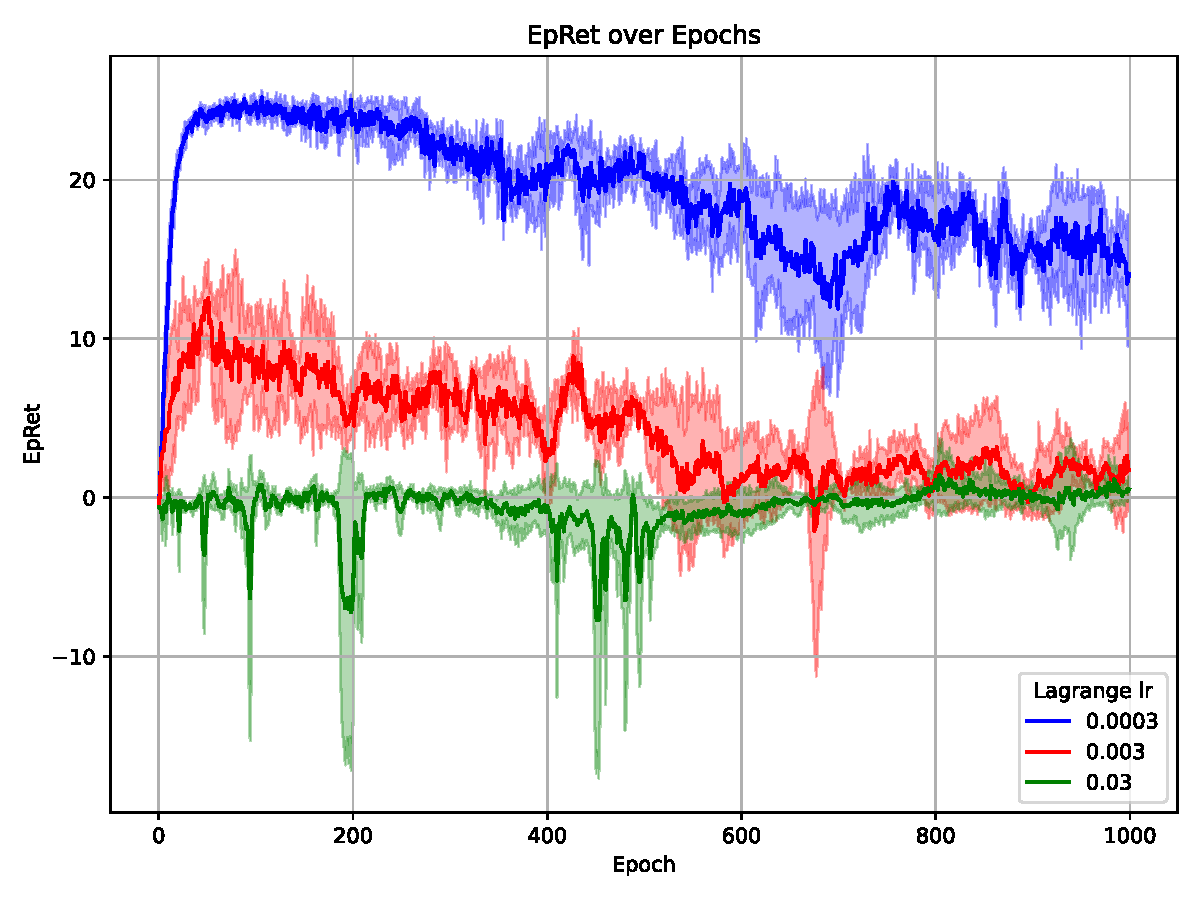
\includegraphics[width=0.65\textwidth]{imgs/chap4/lagrange_lr/return.pdf}
  \caption{Training curves of return over epochs for different learning rate initializations in the Lagrange multiplier network}
  \label{chap4:fig:lagrange_lr_return}
\end{figure*}

\begin{figure*}[h]
  \centering
  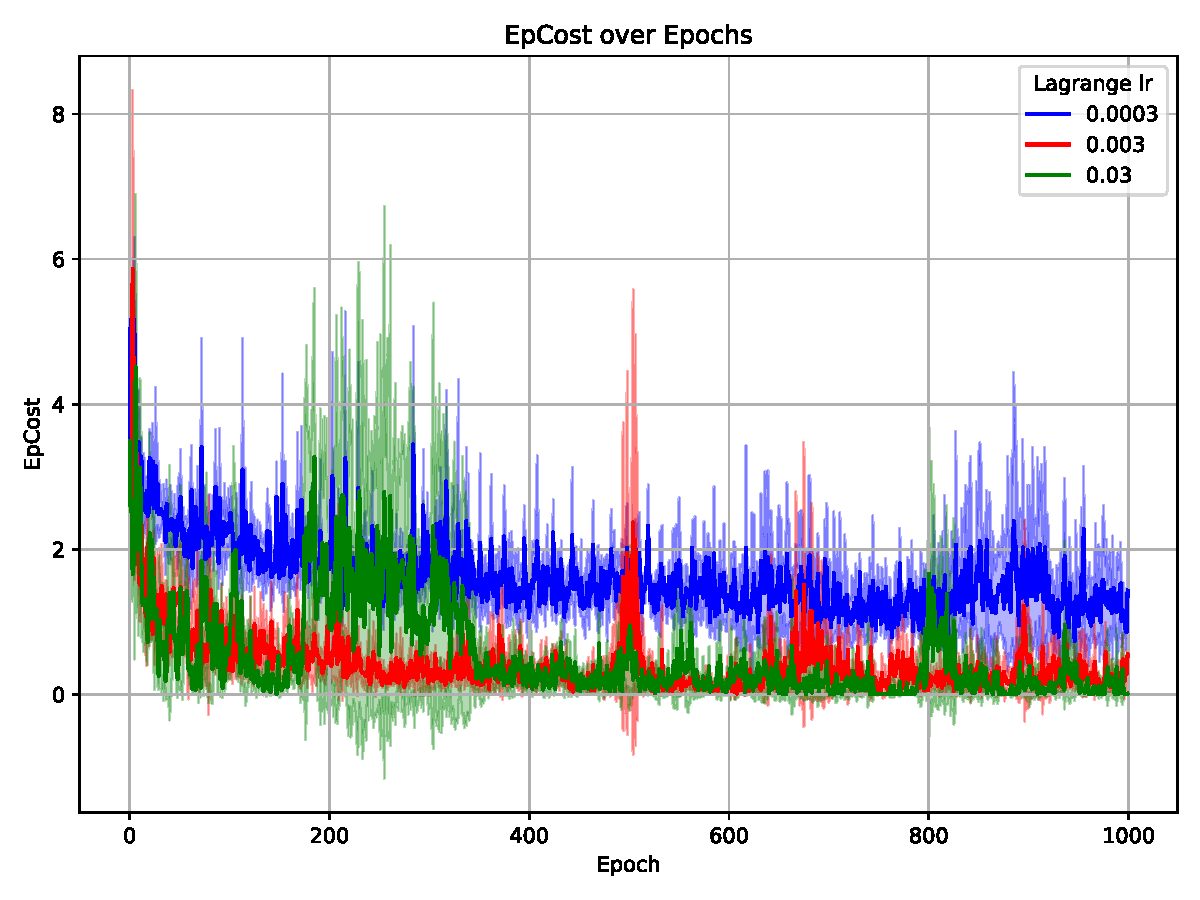
\includegraphics[width=0.65\textwidth]{imgs/chap4/lagrange_lr/cost.pdf}
  \caption{Training curves of cost return over epochs for different learning rate initializations in the Lagrange multiplier network}
  \label{chap4:fig:lagrange_lr_cost}
\end{figure*}

\begin{figure*}[h]
  \centering
  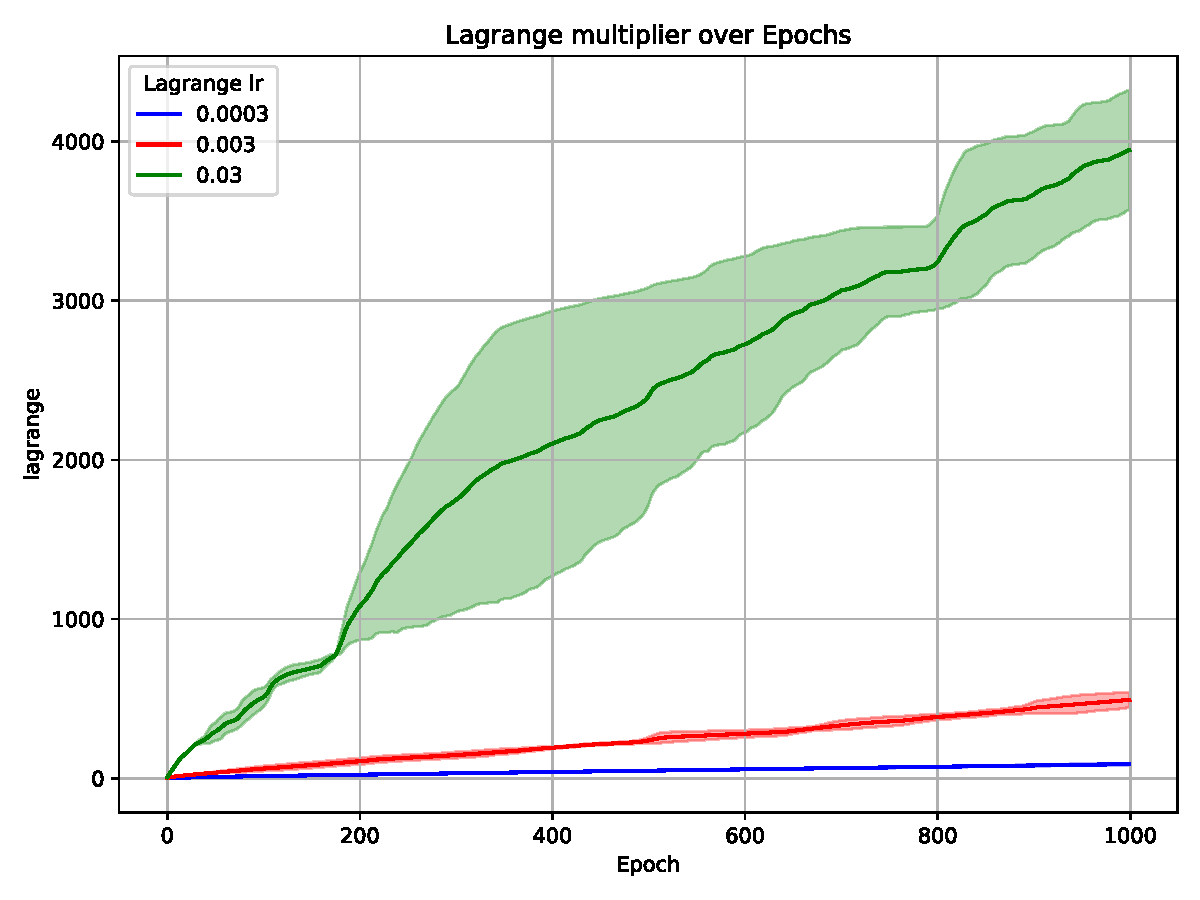
\includegraphics[width=0.65\textwidth]{imgs/chap4/lagrange_lr/lagrange.pdf}
  \caption{Training curves of Lagrange multiplier over epochs for different learning rate initializations in the Lagrange multiplier network}
  \label{chap4:fig:lagrange_lr_lagrange}
\end{figure*}

Fig ~\ref{chap4:fig:lagrange_lr_return} - \ref{chap4:fig:lagrange_lr_lagrange} show the impact of learning rate on return, cost, and the Lagrange multiplier.
Except for the case with a learning rate of 0.0003, all other settings converge to near-zero returns during training.
In the case of a 0.003 learning rate, the return begins to decrease slightly after around epoch 400. During this period, the Lagrange multiplier continued its steady growth, increasing from around 200 at epoch 400 to approximately 500 by epoch 1000.
This suggests that stronger constraint enforcement over time leads to a drop in reward.
With a learning rate of 0.03, the Lagrange multiplier grows rapidly and exhibits high variance, making the overall training highly unstable.
These findings suggest that the learning rate of the Lagrange multiplier network must be carefully tuned to ensure stable training while appropriately enforcing the constraints.
Therefore, in the subsequent experiments, we initialize the bias of the Lagrange multiplier network to 20 and set the learning rate to 0.0003.

\clearpage

\begin{table}[h]
  \centering
  % \caption{Hyperparameters used in Experiment \ref{chap4:sec:experiments:lagrange_init} and \ref{chap4:sec:experiments:lagrange_lr}}
  \caption{Hyperparameters used in Experiments ~\ref{chap4:sec:experiments:lagrange_init} and~\ref{chap4:sec:experiments:lagrange_lr}. In each experiment, either the Lagrange multiplier initialization bias or the learning rate was varied, as shown in the corresponding plots. The other hyperparameter was fixed to the value listed in this table.}
  \label{tab:hyperparams-lagrange-init}
  \begin{tabular}{l c}
    \toprule
    \textbf{Hyperparameter} & \textbf{Value} \\
    \midrule
    Environment                         & Point Goal \\
    Number of epochs                    & 1000 \\
    Number of steps per epoch           & 30000 \\
    Hidden layer size (MLP)             & 64 \\
    gamma (discount factor)             & 0.99 \\
    lambda (GAE)                        & 0.97 \\
    Learning rate (policy)              & 3e-4 \\
    Learning rate (value function)      & 1e-3 \\
    Learning rate (Lagrange multiplier) & 3e-4 \\
    Lagrange multiplier init (bias)     & 0 \\
    \bottomrule
  \end{tabular}
\end{table}

%%%%%%%%%%%%%%%%%%%%%%%%%%%%%%%%
\section{Evaluation Results}
%%%%%%%%%%%%%%%%%%%%%%%%%%%%%%%%

In this section, we present the a comparative evaluation of PPO Lagrangian, Feasible Actor-Critic, and our proposed method across two tasks: Car Goal, and Car Button.

\subsection{Car Goal} \label{chap4:sec5:car_goal}

In the Car Goal task, we compare the performance of Feasible Actor-Critic (FAC), PPO Lagrangian, and our proposed PPO Lagrangian Network (PPO-Lagnet).
As shown in Fig.~\ref{chap4:fig:car_goal_return}, all three methods converge to similar return values, indicating comparable task performance in terms of reward.
In terms of cost return (Fig.~\ref{chap4:fig:car_goal_cost}), both PPO-based methods (PPO Lagrangian and PPO-Lagnet) show stable and consistent reductions in cost over time.
In contrast, the FAC method produces highly fluctuating cost values throughout training.
In addition, as shown in Fig.~\ref{chap4:fig:car_goal_return}, the FAC method exhibits higher variance in return compared to the PPO-based methods.
This instability may be caused by a conflict between SAC’s entropy regularization and the penalty term introduced by the Lagrange multiplier.
While entropy regularization encourages exploration, the penalty term enforces constraint satisfaction, which can lead to conflicting optimization objectives.
These factors make the FAC method more sensitive to hyperparameter choices and appear to result in lower stability compared to the on-policy PPO-based approaches.
Finally, as shown in Fig.~\ref{chap4:fig:car_goal_lagrange}, we can observe that the Lagrange multiplier network in the FAC method was initialized with zero bias, as large initial values were found to cause unstable learning dynamics in preliminary experiments.
Additionally, we note that this experimental result differs from the one reported in the FAC paper.
As mentioned in Section~\ref{chap4:sec:setup}, we use a dense cost formulation, where the actual cost values vary depending on the state.
In contrast, the FAC implementation uses a sparse cost formulation, where the agent receives a cost of 1 if a constraint is violated and 0 otherwise.
This leads to differences in the learned Q-function and cost Q-function values, potentially resulting in different optimization process and constraint enforcement behavior.

\begin{figure*}[h]
  \centering
  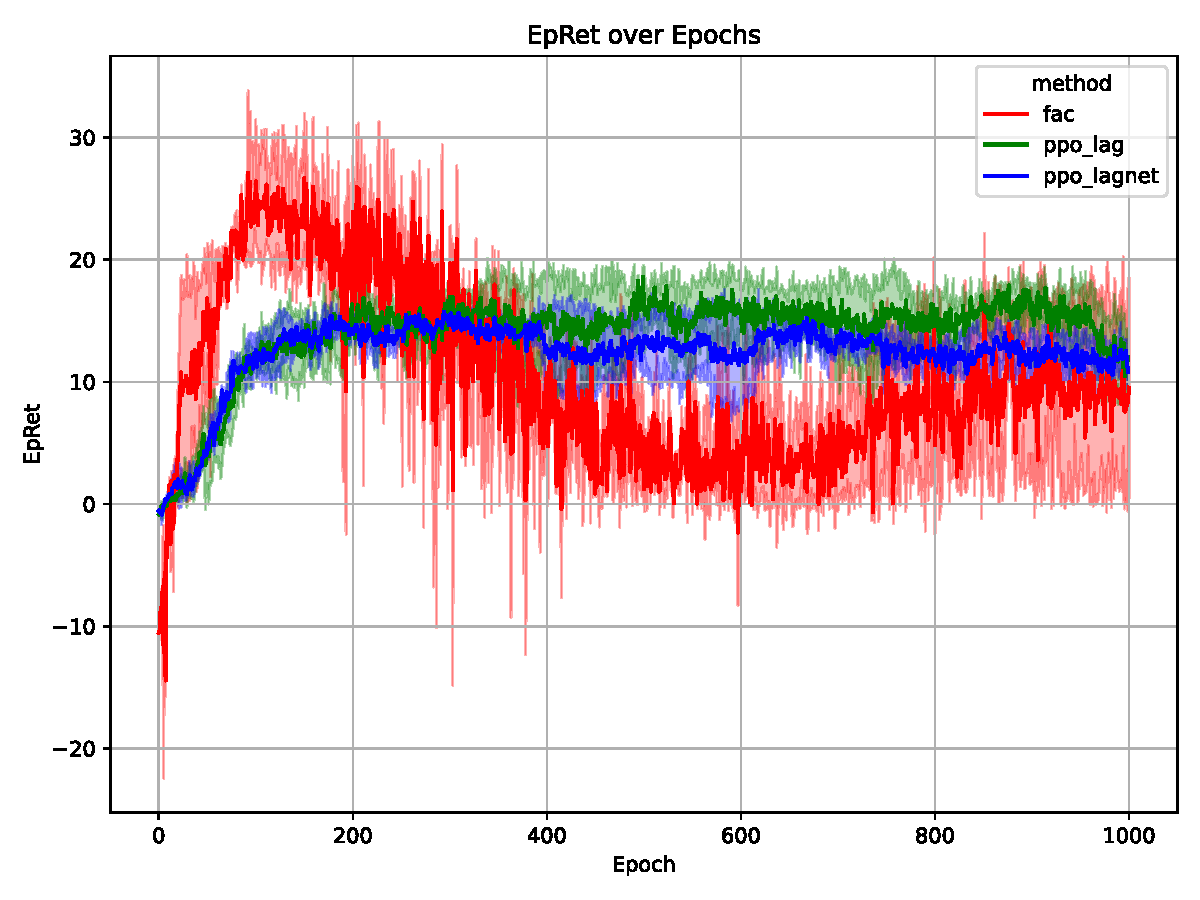
\includegraphics[width=0.65\textwidth]{imgs/chap4/car_goal/return.pdf}
  \caption{Training curves of return over epochs for PPO Lagrangian, Feasible Actor-Critic, and PPO Lagrangian Network on the Car Goal task}
  \label{chap4:fig:car_goal_return}
\end{figure*}

\begin{figure*}[h]
  \centering
  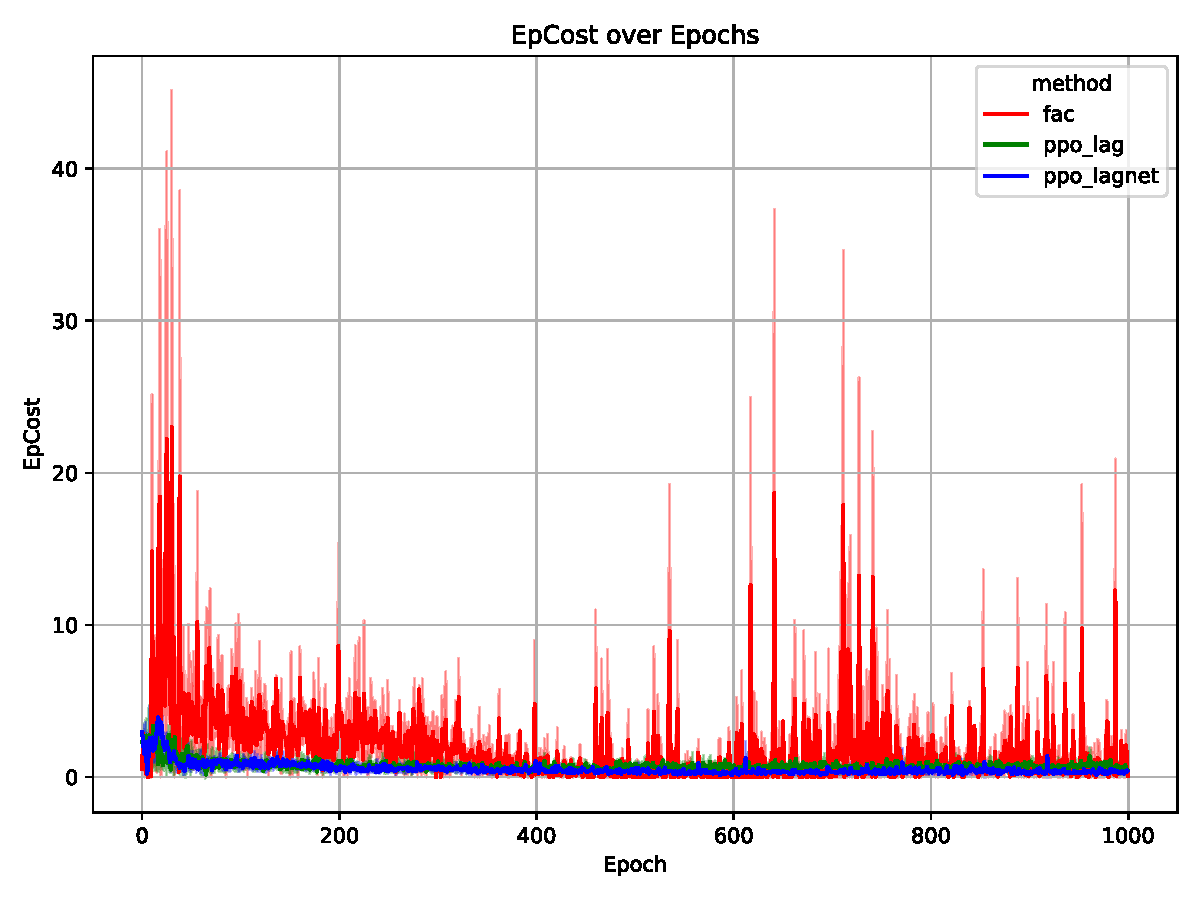
\includegraphics[width=0.65\textwidth]{imgs/chap4/car_goal/cost.pdf}
  \caption{Training curves of cost return over epochs for PPO Lagrangian, Feasible Actor-Critic, and PPO Lagrangian Network on the Car Goal task}
  \label{chap4:fig:car_goal_cost}
\end{figure*}

\clearpage

\begin{figure*}[t]
  \centering
  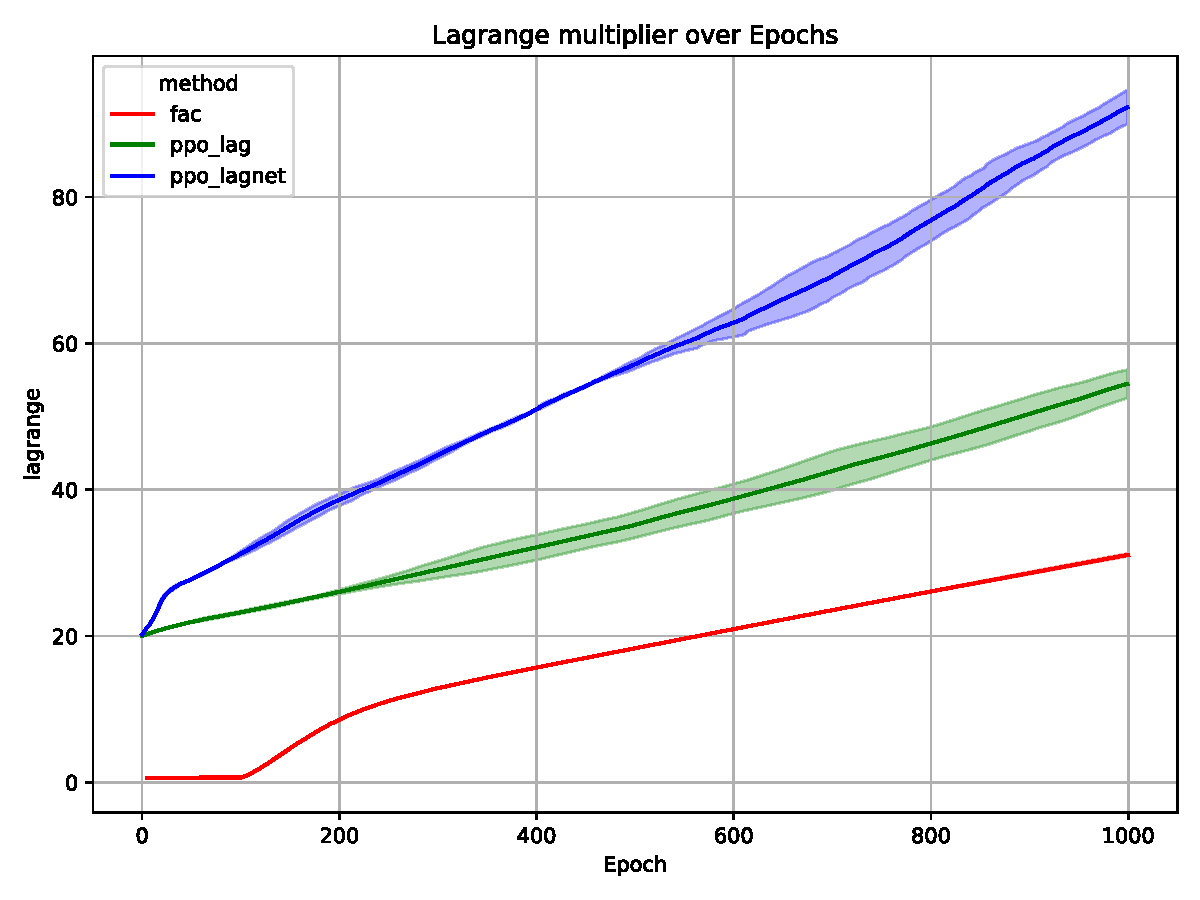
\includegraphics[width=0.65\textwidth]{imgs/chap4/car_goal/lagrange.pdf}
  \caption{Training curves of Lagrange multiplier over epochs for PPO Lagrangian, Feasible Actor-Critic, and PPO Lagrangian Network on the Car Goal task}
  \label{chap4:fig:car_goal_lagrange}
\end{figure*}


\subsection{Car Button}

Unlike the Car Goal task discussed in Section~\ref{chap4:sec5:car_goal}, this task contains more obstacles, which makes policy learning difficult when the cost limit is set to zero (i.e., when any constraint violation is strictly prohibited).
Therefore, in this task, we set the state-wise allowable cost to 0.3, which corresponds to allowing a maximum cumulative cost of 300 per episode (given the episode length is fixed at 1000 steps).
Additionally, since setting the Lagrange multiplier network’s bias to 20 resulted in unstable learning in this task, we initialized it with zero bias in this experiment.
As shown in Fig.~\ref{chap4:fig:car_button_return}, our proposed method demonstrates stable convergence in return.
In contrast, the PPO Lagrangian method (green) shows unstable policy behavior between epochs 300 and 600, followed by performance recovery in the later stages.
For the FAC method, the policy does not improve until around epoch 800, and only starts to receive meaningful rewards after epoch 900.
Looking at Fig.~\ref{chap4:fig:car_button_cost}, we observe that the cost values of FAC begin to increase around the same time its return starts to improve.
These results indicate that FAC needs more training iterations in this task to effectively balance reward acquisition and constraint satisfaction.
Both PPO-based methods (PPO Lagrangian and our proposed method) appear to satisfy the constraints effectively, and in particular, our proposed method maintains stable constraint satisfaction starting from around epoch 100.

\begin{figure*}[h]
  \centering
  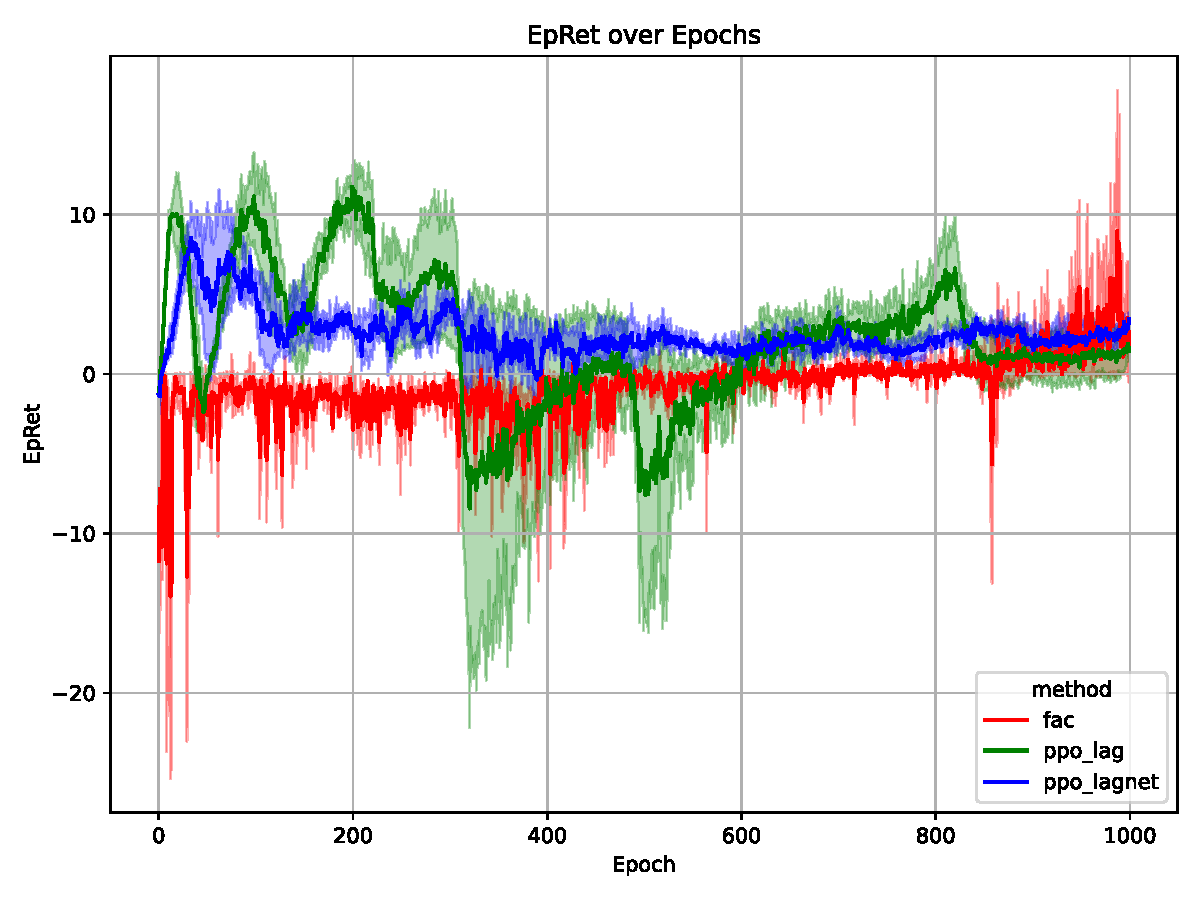
\includegraphics[width=0.7\textwidth]{imgs/chap4/car_button/return.pdf}
  \caption{Training curves of return for PPO Lagrangian, Feasible Actor-Critic, and PPO Lagrangian Network in Car Button task}
  \label{chap4:fig:car_button_return}
\end{figure*}

\begin{figure*}[h]
  \centering
  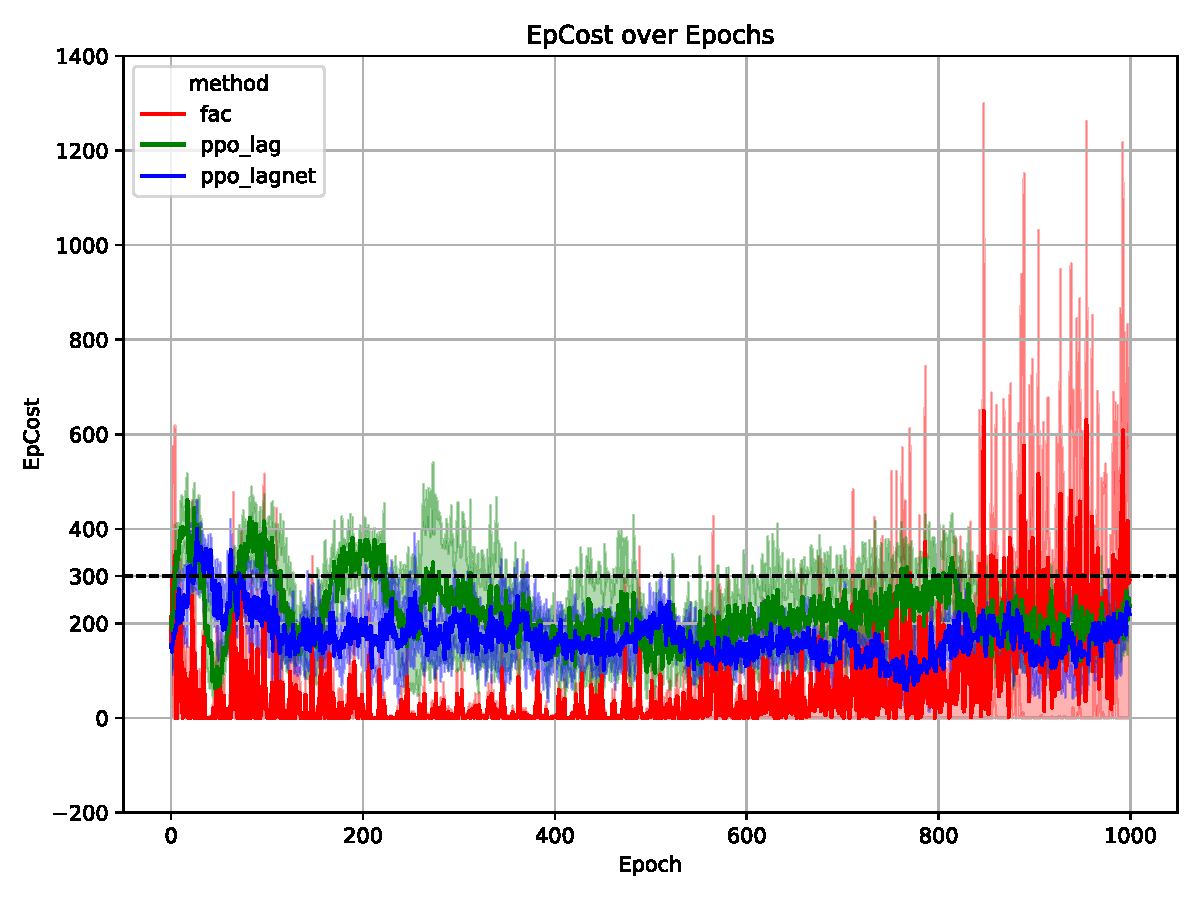
\includegraphics[width=0.7\textwidth]{imgs/chap4/car_button/cost.pdf}
  \caption{Training curves of cost return for PPO Lagrangian, Feasible Actor-Critic, and PPO Lagrangian Network in Car Button task}
  \label{chap4:fig:car_button_cost}
\end{figure*}

\begin{figure*}[h]
  \centering
  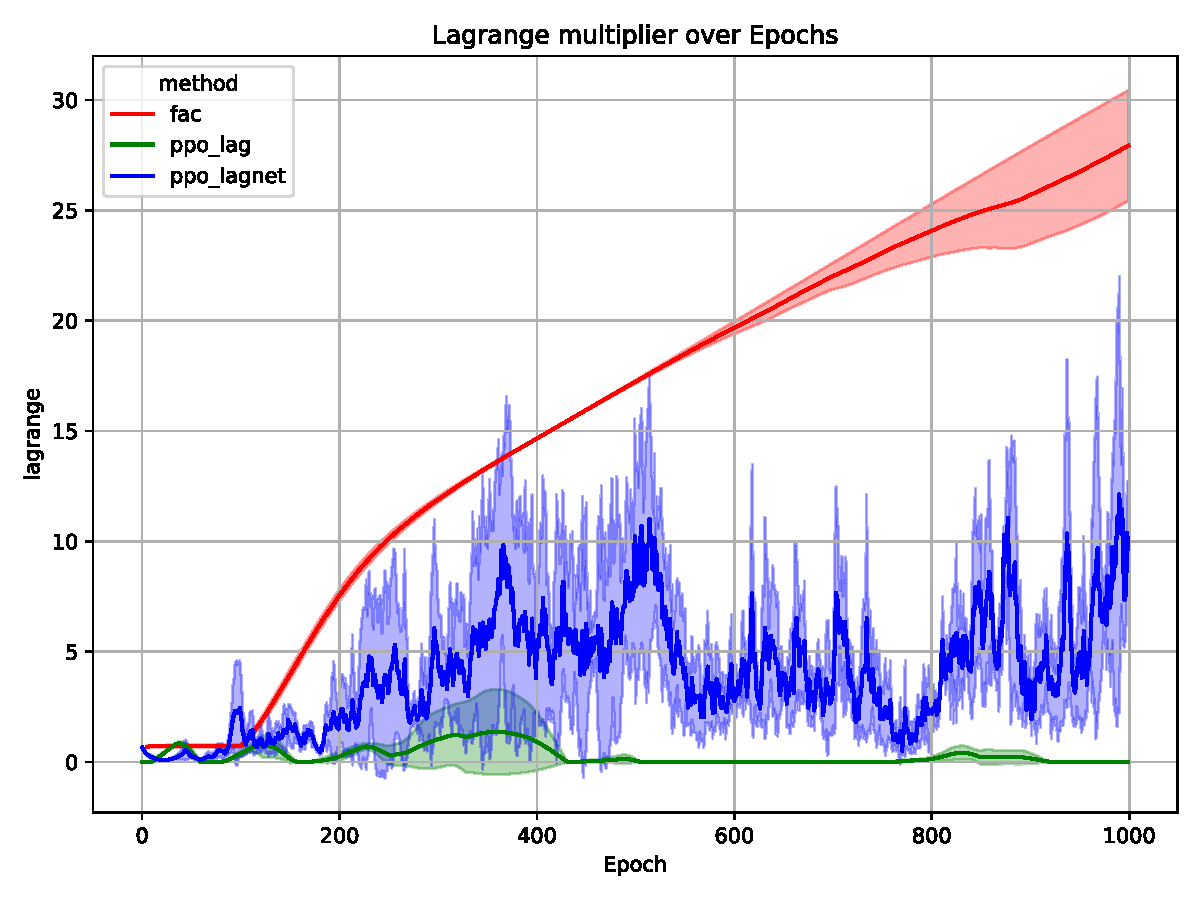
\includegraphics[width=0.7\textwidth]{imgs/chap4/car_button/lagrange.pdf}
  \caption{Training curves of Lagrange multiplier for PPO Lagrangian, Feasible Actor-Critic, and PPO Lagrangian Network in Car Button task}
  \label{chap4:fig:car_button_lagrange}
\end{figure*}

\clearpage

%%%%%%%%%%%%%%%%%%%%%%%%%%%%%%%%
\section{Evaluation Lagrange Multiplier Network}
%%%%%%%%%%%%%%%%%%%%%%%%%%%%%%%%

In this section, we evaluate the performance of the Lagrange multiplier network trained in the Point Goal task.
We utilize the trained Lagrange multiplier network at test time, thereby enabling the assessment of whether the current state is potentially unsafe.
As illustrated in Fig.~\ref{chap4:fig:lagrange_test1} and Fig.~\ref{chap4:fig:lagrange_test2}, the trained Lagrange multiplier network outputs (displayed in the top-right corner of each figure) near-zero or low values when the agent is in a safe state, meaning there are no nearby obstacles or the agent is not moving toward hazardous regions.
As the agent approaches obstacles, the output of the network gradually increases, indicating a higher level of potential risk.
These results demonstrate that the Lagrange multiplier network has successfully learned to assign appropriate penalties based on the agent’s proximity to unsafe areas.
Therefore, it can be effectively used at test time to assess the safety of a given state.

\begin{figure*}[h]
  \centering
  \subfloat[Step 2170]{%
    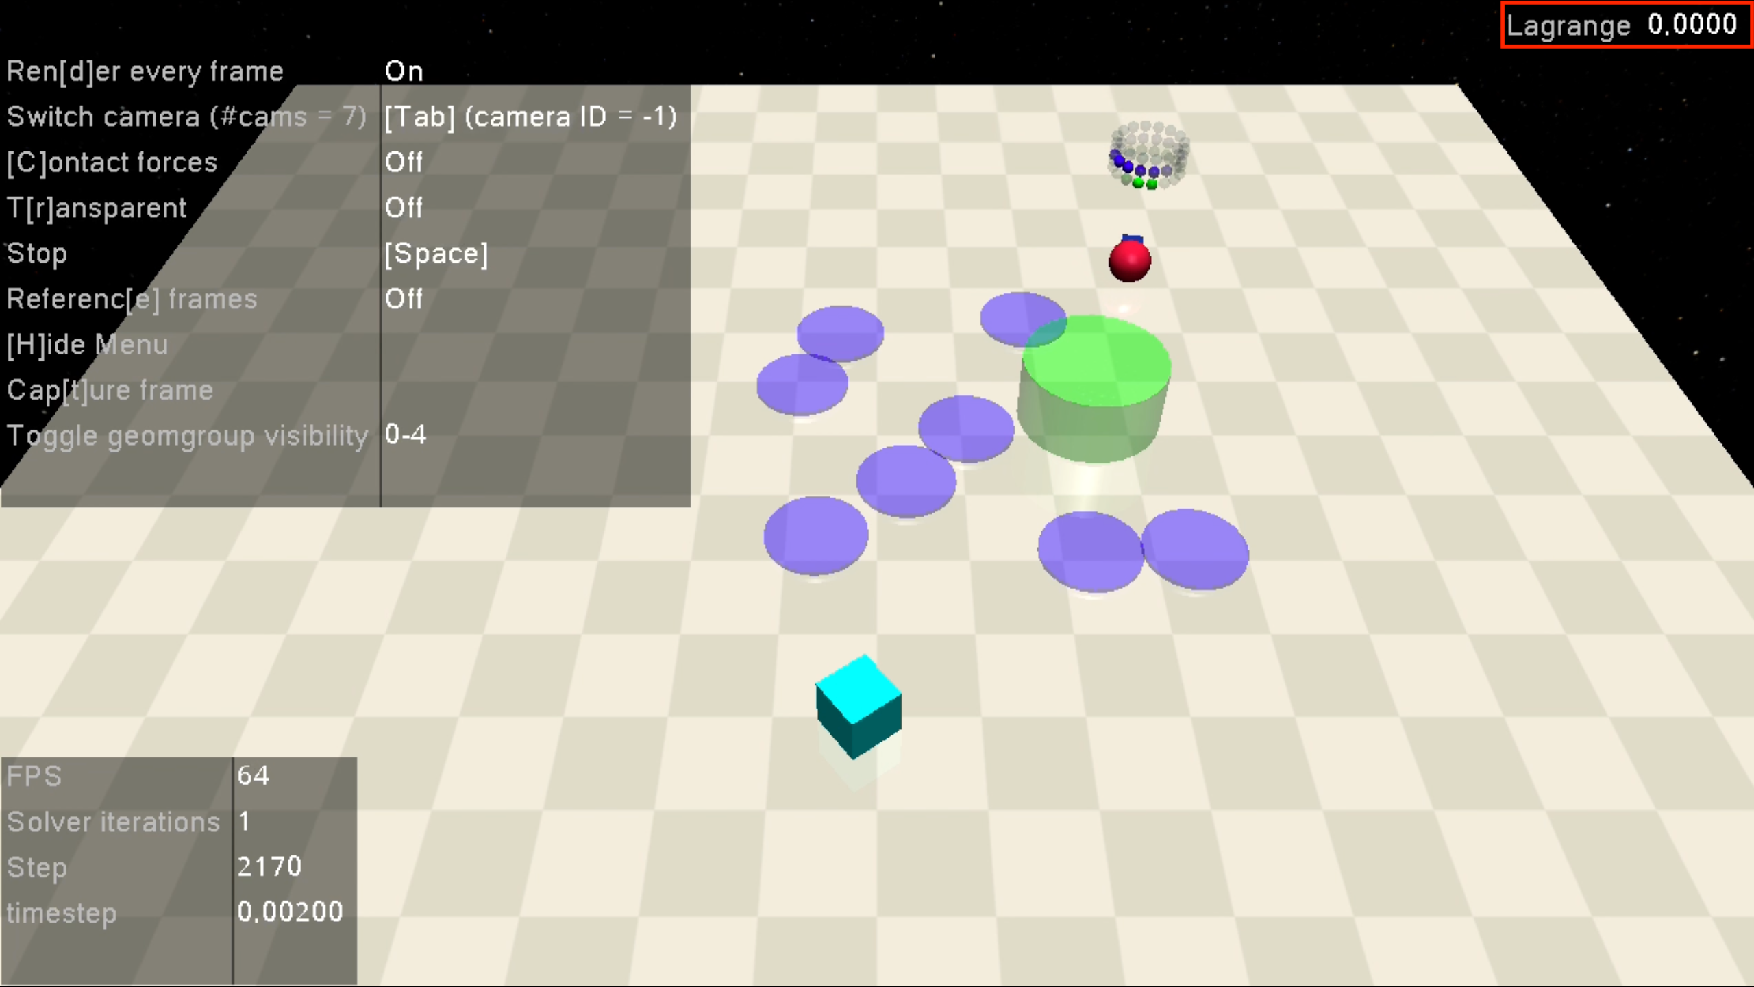
\includegraphics[width=0.7\textwidth]{imgs/chap4/lagrange/test1/0.pdf}
  }

  \vspace{0.2em}

  \subfloat[Step 2450]{%
    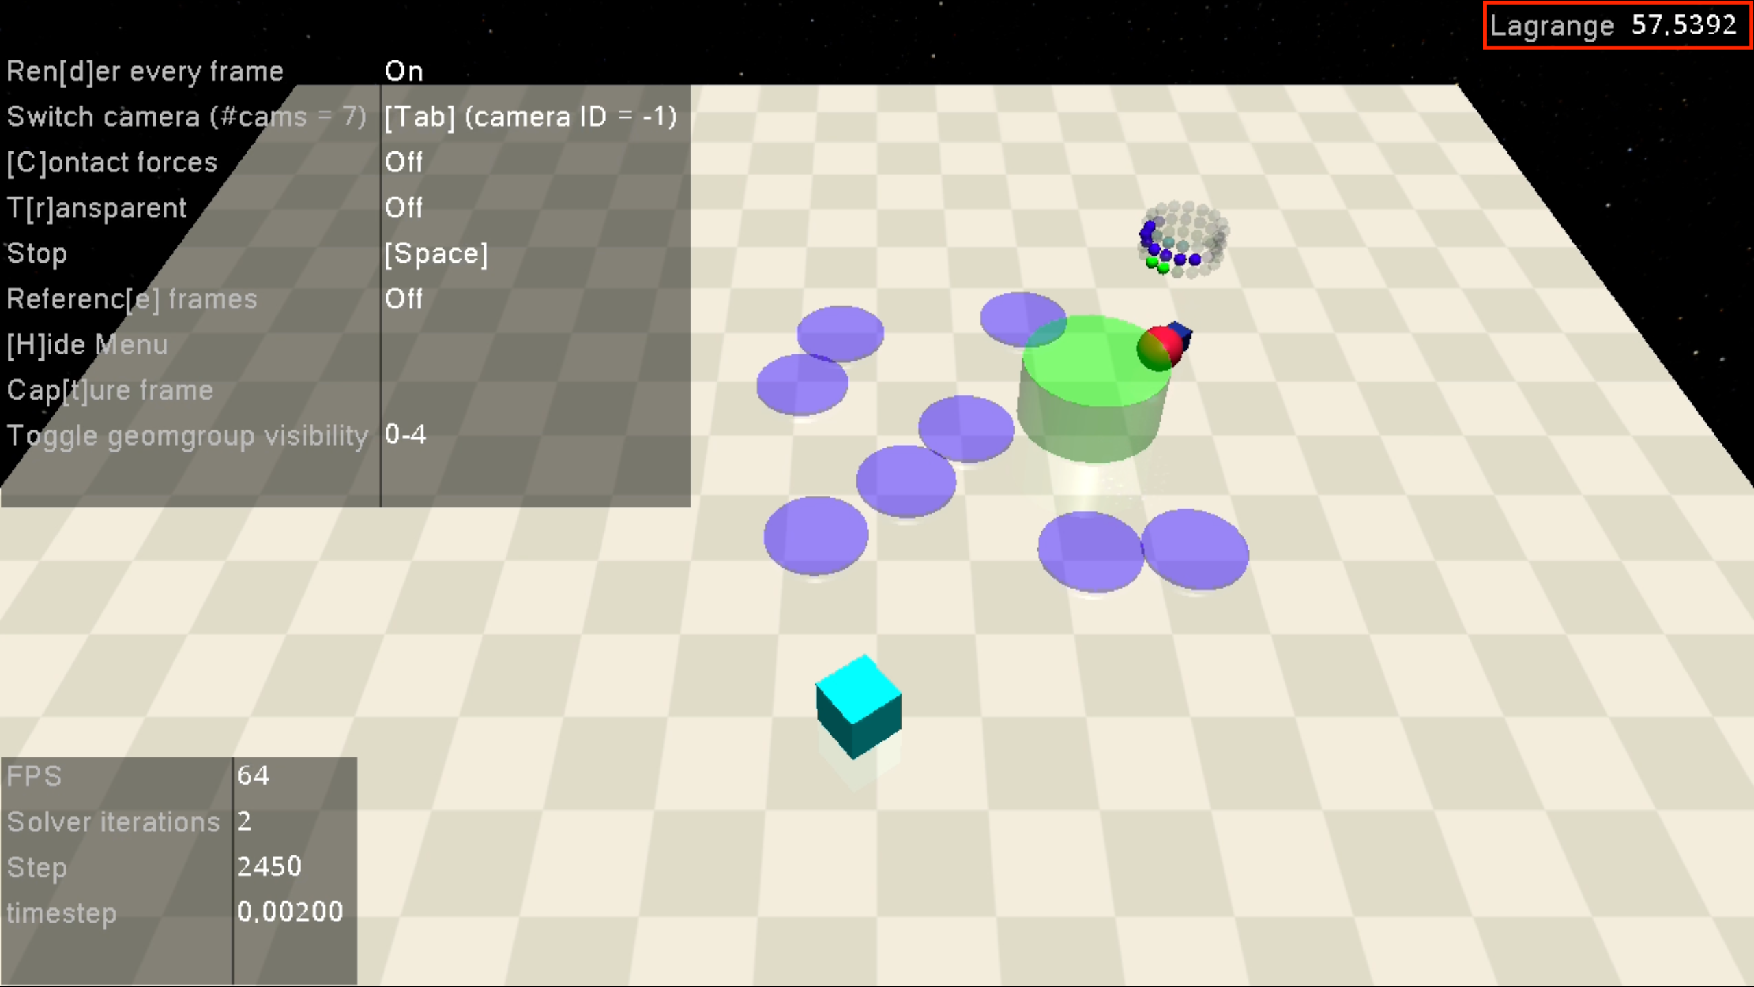
\includegraphics[width=0.7\textwidth]{imgs/chap4/lagrange/test1/50.pdf}
  }

  \vspace{0.2em}

  \subfloat[Step 2670]{%
    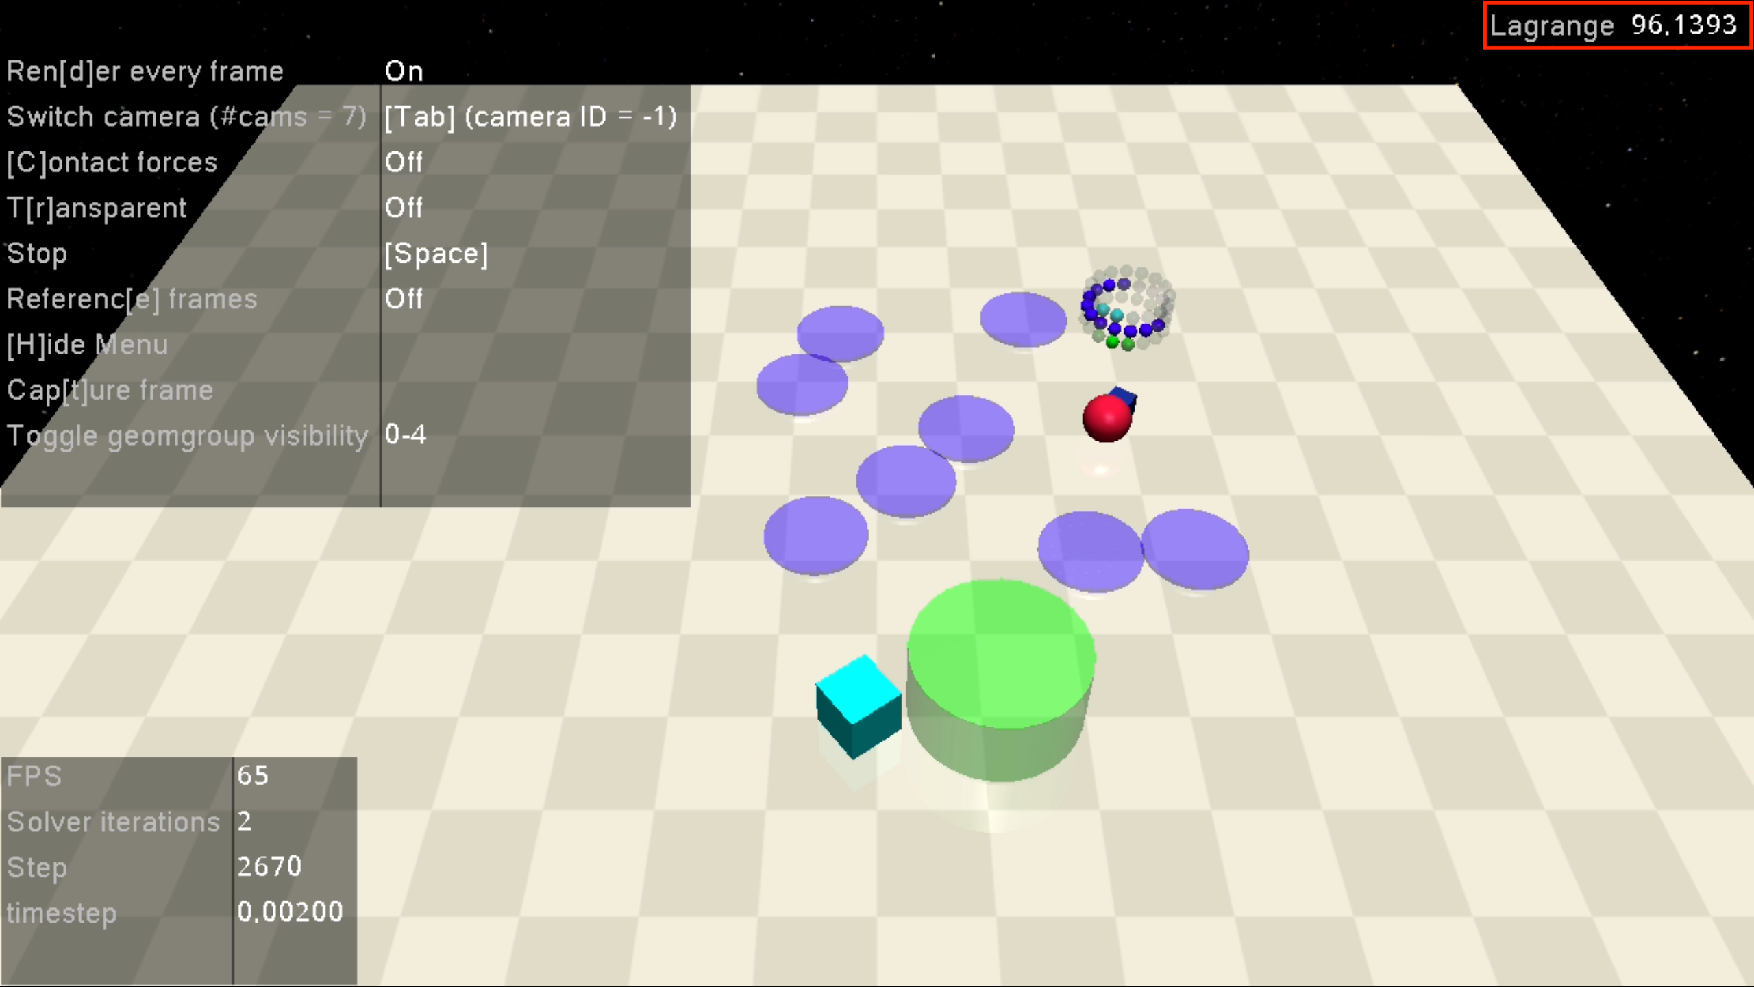
\includegraphics[width=0.7\textwidth]{imgs/chap4/lagrange/test1/90.pdf}
  }

  \caption{Visualization of the Lagrange multiplier network output at different steps in the test scenario 1}
  \label{chap4:fig:lagrange_test1}
\end{figure*}

\begin{figure*}[h]
  \centering
  \subfloat[Step 4640]{%
    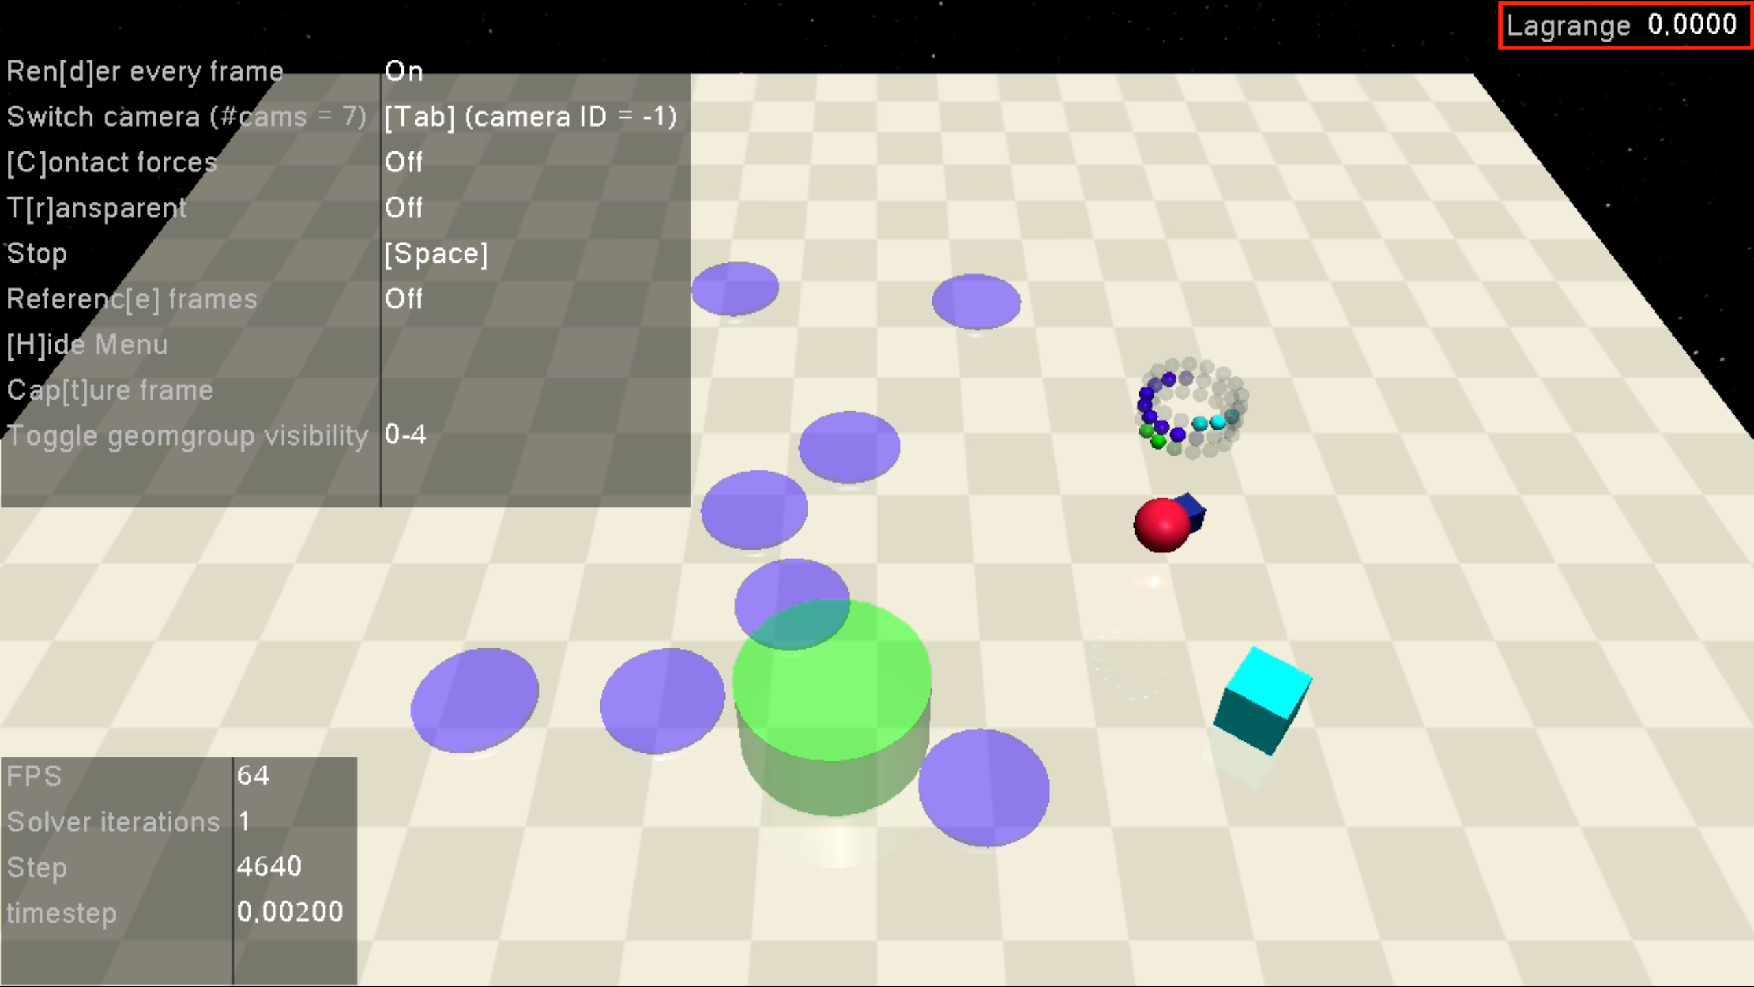
\includegraphics[width=0.7\textwidth]{imgs/chap4/lagrange/test2/0.pdf}
  }

  \vspace{0.2em}

  \subfloat[Step 4850]{%
    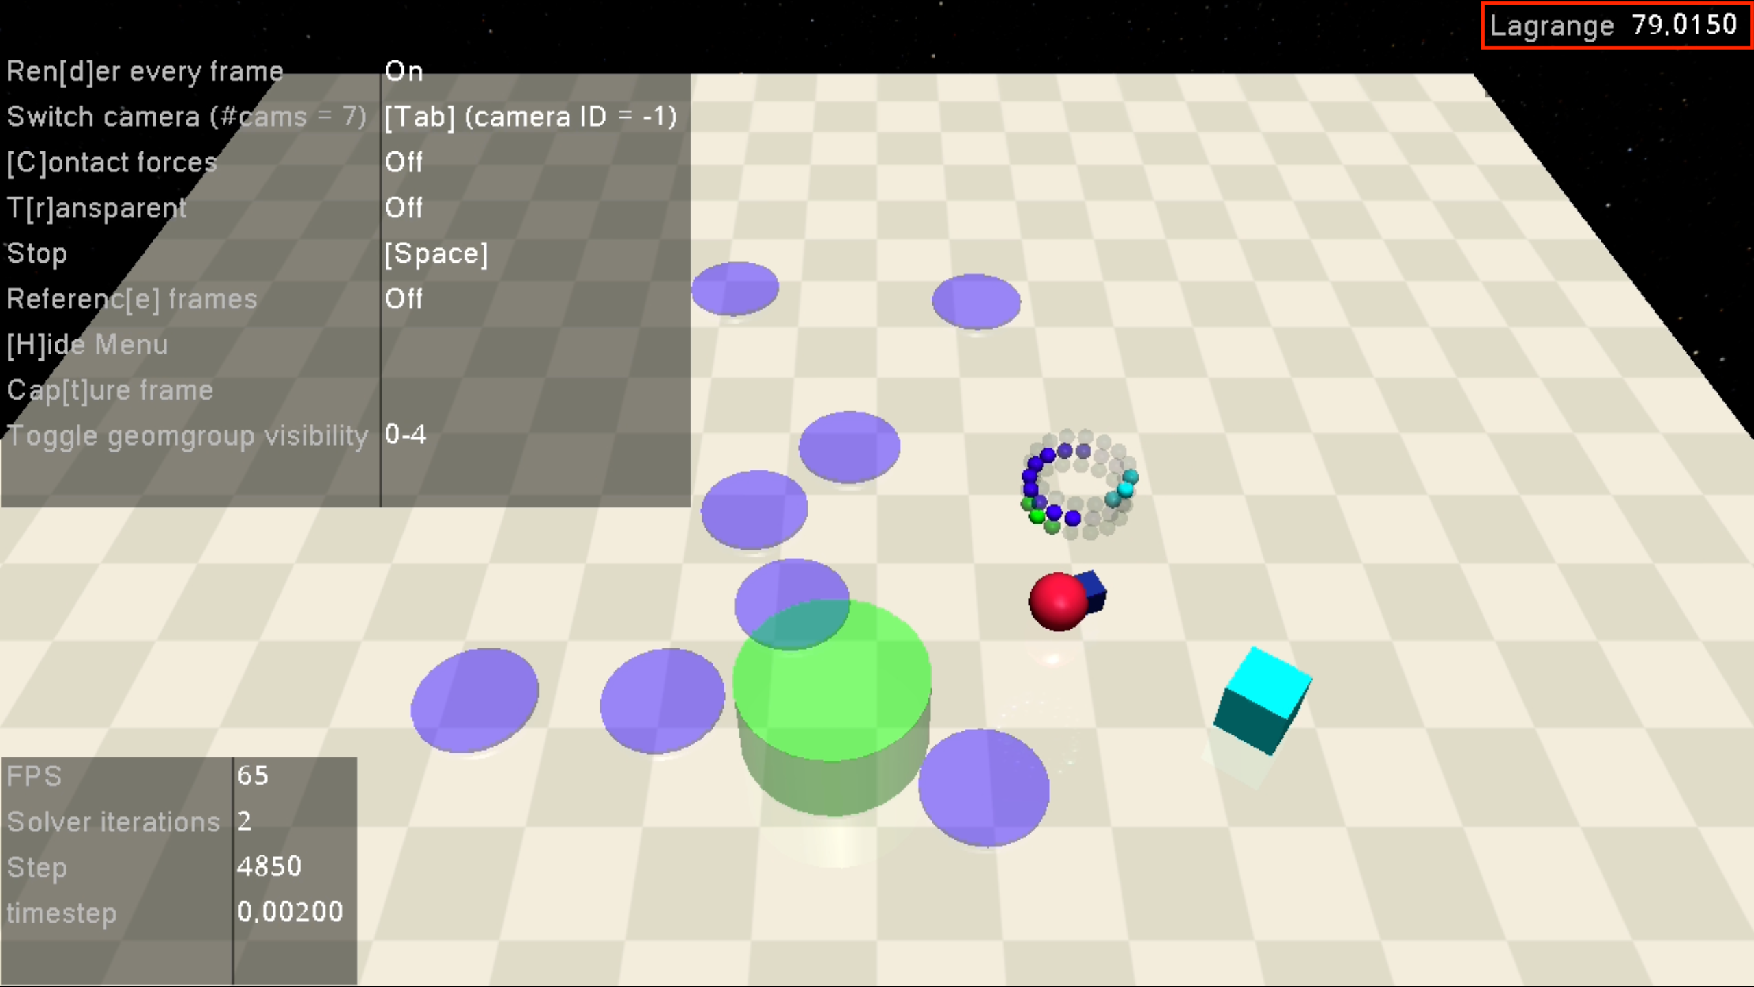
\includegraphics[width=0.7\textwidth]{imgs/chap4/lagrange/test2/80.pdf}
  }

  \caption{Visualization of the Lagrange multiplier network output at different steps in the test scenario 2}
  \label{chap4:fig:lagrange_test2}
\end{figure*}

\end{spacing}

%%%%%%%%%%%%%%%%%%%%%%%%%%%%%%%%%%%%
% Chapter 5
%%%%%%%%%%%%%%%%%%%%%%%%%%%%%%%%%%%%

\begin{spacing}{2.0} % double spacing
  
%%%%%%%%%%%%%%%%%%%%%%%%%%%%%%%%
% Chap 5. Conclusion
%%%%%%%%%%%%%%%%%%%%%%%%%%%%%%%%

\chapter{Conclusion}\label{chapter5}

\section{Conclusion}

In this thesis, we proposed an extension to Proximal Policy Optimization (PPO) by incorporating a Lagrange multiplier network, enabling the policy to account for state-wise constraints during training.
This method incorporates a network that estimates state-wise Lagrange multipliers to enforce safety constraints at the state level, allowing for more flexible and precise control over the policy's behavior in constrained environments.
We conducted an empirical analysis of the impact of the bias initialization and learning rate on the performance of the Lagrange multiplier network.
Our experiments show that setting the bias in the range of 0 to 20 and using a learning rate similar to that of the policy network yields the most stable and effective learning outcomes.
Furthermore, when compared to existing methods such as PPO Lagrangian and Feasible Actor-Critic, our proposed approach exhibited more consistent and reliable constraint satisfaction across different tasks.
These results suggest that our method provides a robust framework for safe reinforcement learning under state-wise constraints.
We also found that the trained Lagrange multiplier network can be deployed at test time to assess whether the current state is potentially unsafe.
If the network outputs a high value for a given state, it typically indicates that the agent is near a constraint-violating region (e.g., close to an obstacle).
In such cases, we observed that the agent adjusts its behavior to avoid hazards and navigates more safely.

\section{Limitations and Future Work}

While our proposed method demonstrates promising results in enforcing state-wise constraints, several limitations remain.
First, since the policy is trained to satisfy constraints by incorporating penalty terms, it does not offer deterministic safety guarantees.
Even after training, constraint violations may still occur.
To overcome this issue, the trained Lagrange multiplier network can be leveraged at test time to identify high-risk situations.
If an action is considered unsafe, a safety filter may be used to override it, thereby improving safety at deployment.
Moreover, while our method does not guarantee stability during training, this limitation may be addressed by integrating techniques that ensure safe exploration.
For example, projection-based approaches \cite{CPO, PCPO}, which optimize the policy while keeping it within the feasible region, could be considered.
Second, our current evaluation is restricted to the relatively simple Safety Gym environments implemented using the MuJoCo engine.
To further validate the practicality and generalizability of our approach, we plan to extend our experiments to more realistic and safety-critical domains, such as CARLA \cite{CARLA}, a high-fidelity autonomous driving simulator.
This transition would enable us to evaluate the robustness, scalability, and real-world applicability of the proposed method in more complex and dynamic scenarios.

\end{spacing}

      
%%%%%%%%
% Add more chapters if you wants
%%%%%%%%


%---------
% summary
%---------
\begin{spacing}{2.0}

\summary

This thesis studies how to train policies to satisfy state-wise safety using state-wise constrained reinforcement learning.
We focus on Lagrangian-based approaches and identify their key limitations, particularly with respect to stability and convergence.
To address these challenges, we propose PPO Lagrangian Network, an extension of Proximal Policy Optimization that incorporates a Lagrange multiplier network to dynamically enforce safety constraints at the state level.
Extensive experiments on the OpenAI Safety Gym benchmark show that proposed method achieves more stable and reliable constraint satisfaction than existing approaches such as PPO Lagrangian and Feasible Actor-Critic (FAC).
We further investigate how hyperparameter choices, such as the initialization bias and learning rate of the Lagrange multiplier network, affect performance.
Our findings indicate that careful tuning of these parameters is crucial for maintaining stability under hard constraint settings.
Additionally, we demonstrate that the trained Lagrange multiplier network can be reused at test time as a risk estimator, allowing the agent to assess the safety of a given state and adjust its behavior accordingly.
\end{spacing}

%-----------------------------------------------------------------------
% This is the end of the main thesis body.

%-----------------------------------------------------------------------
% Input the list of references.
\bibliographystyle{ieeetr}
\bibliography{biblist}

%%%%%%%%%%%%%%%%%%%%%%%%%%%%%%%%%%%%%%%%%%%%%%%%
% Appendix
% You can comment out if you do not need appendix
%%%%%%%%%%%%%%%%%%%%%%%%%%%%%%%%%%%%%%%%%%%%%%%%
% \begin{spacing}{2.0}
% 
%%%%%%%%%%%%%%%%%%%%%%%%%%%%%%%%%%%%%%%%%%%%%%%%
% Appendix
%%%%%%%%%%%%%%%%%%%%%%%%%%%%%%%%%%%%%%%%%%%%%%%%

%\appendixpage
\appendix

\chapter{Abbreviations}
%%% define some Abbreviations
\text{ } \text{ }  \textbf{GIST} \text{ } \text{ } Gwangju Institute of Science and Technology

\textbf{EECS}  \text{ } \text{ } Electrical Engineering and Computer Science

\textbf{YOLO}  \text{ } \text{ } You Only Live Once



\chapter{More appendix}

You can add more appendices.
% \end{spacing}

%-----------------------------------------------------------------------
% Acknowledgements
% Insert the text between \begin{acknowledgements} and \end{acknowledgements}.
% You can either write the abstract directly here or import a file using the \input command.

%%%%%%%%%%%%%%%%%%%%%%%%%%%%%%%%%%%%%%%%%%
% Acknowledgements by Korean
%%%%%%%%%%%%%%%%%%%%%%%%%%%%%%%%%%%%%%%%%%
\begin{acknowledgements}
\begin{spacing}{2.0}
%%%%%%%%%%%%%%%%%%%%%%%%%%%%%%%%%%%%%%
% Acknowledgements of the thesis in English
%%%%%%%%%%%%%%%%%%%%%%%%%%%%%%%%%%%%%%
\end{spacing}
\end{acknowledgements}


%-----------------------------------------------------------------------
% Input the curriculum vitae.
% You may add as many lines as you need using the syntax of the \item command shown below.
%-----------------------------------------------------------------------



%\input Vitae2.0.tex
%\input thesis-publications.tex

% Insert activity if you have.
%\activity
%Activity Activity Activity Activity Activity Activity Activity Activity
%Activity Activity Activity Activity Activity Activity Activity Activity

% Insert awards if you have.

%-----------------------------------------------------------------------
% This is the end of the thesis.
%
\end{document}
